\documentclass[letter,11pt]{article}
\usepackage[spanish, activeacute]{babel}
\usepackage{amsfonts}
\usepackage{amsmath,amsfonts,amssymb}
\usepackage{fancyhdr}
\usepackage{fancyvrb}
\usepackage{xy}
\usepackage{graphicx}
\usepackage{latexsym,amsfonts}
\usepackage{enumerate}
\usepackage{multirow}
\usepackage{multicol}
\usepackage{hyperref}
\usepackage{longtable}
\usepackage{hyperref}
\hypersetup{
    colorlinks=true,       % false: boxed links; true: colored links
    linkcolor=red,          % color of internal links (change box color with linkbordercolor)
}
\usepackage[numbered,framed]{matlab-prettifier}
\lstMakeShortInline"
\lstset{
  style              = Matlab-editor,
  escapechar         = ",
  mlshowsectionrules = true,
  morekeywords={endif,endfor,endwhile},
}

\setlength{\oddsidemargin}{-0.5cm}
\setlength{\evensidemargin}{0cm}
\setlength{\textwidth}{17.5cm}
\setlength{\textheight}{24cm}
\setlength{\topmargin}{-1.7cm}

\title{lab06 521230 2018-2}

\font\bff=cmbx10 at 10truept
\font\lg=cmdunh10 at 10truept
\font\bl=cmss10 at 10truept

\newcommand{\matlab}{{\sc Matlab} }
\newcommand{\octave}{{\sc Octave} }

\newcommand{\header}{\noindent%
{\lg UNIVERSIDAD DE CONCEPCI\'ON}\hfill
\vskip-4truept
\noindent{\bff FACULTAD DE CIENCIAS}\hfill
\vskip-4truept
\noindent{\bff F\'ISICAS Y MATEM\'ATICAS}\hfill
\vskip-4truept
\noindent{\bl DEPARTAMENTO DE INGENIER\'IA MATEM\'ATICA}\hfill
\vskip4truept\hrule\hrule\vskip4truept
\par
}


\begin{document}
\header
\vspace{0.7cm}
\begin{center}
\textbf{\small C\'alculo Num\'erico (521230) - Laboratorio 6}\\
\vspace{0.1cm}
\textbf{\Large PROBLEMAS DE ECUACIONES DIFERENCIALES EN OCTAVE}
\vspace{0.7cm}
\end{center}


\section{EDO y PVI}
Una ecuaci\'on diferencial ordinaria (EDO) de primer orden junto a la exigencia de que la funci\'on soluci\'on pase por un punto en particular de denomina problema de valores iniciales (PVI).
Un PVI gen\'erico tiene la forma
$$
\begin{array}{c|}
y'(x)=f(x,y(x)),\\
y(x_0)=y_0.\\
\hline
\end{array}
$$
Los ejemplos
$$
\begin{array}{c|}
y'(x)=y(x)\\
y(0)=1\\
\hline
\end{array}\,,
\quad 
\begin{array}{c|}
y'(x)=\sen(x)\\
y(1)=2\\
\hline
\end{array}\,,
\quad 
\begin{array}{c|}
y'(x)=\cos(x)+y(x)\\
y(-1)=1\\
\hline
\end{array}\,,
$$
son PVI de orden uno. Estos problemas tienen por soluci\'on funciones de una variable $y$ que deben satisfacer simult\'aneamente su EDO y su condici\'on inicial.

Una EDO se dice de orden superior si involucra derivadas de orden mayor o igual que dos en su expresi\'on. Por ejemplo
$$
y''(x)+P(x)y(x)=F(x)
$$
es una EDO de orden dos. Mediante sustituciones toda EDO de orden superior se puede reescribir como un sistema de EDO de orden uno. A modo de ejemplo la EDO
$$
\begin{array}{c|}
2x''(t)-x'(t)-3x(t)=\cos(t) \\
\hline
\end{array}
$$
se transforma en el sistema
$$
\begin{bmatrix}
u_1(t)\\
u_2(t)
\end{bmatrix}'
=
\begin{bmatrix}
u_2(t) \\
\frac{\cos(t)+3u_1(t)+u_2(t)}{2}
\end{bmatrix}
$$
mediante la sustituci\'on
$u_1(t)=x(t)$ y $u_2(t)=x'(t)$.

\subsection{Soluci\'on num\'erica de PVI}
Entendemos por soluci\'on num\'erica de un PVI como una colecci\'on de puntos $(x_0, y_0), \dotsc, (x_n,y_n)$ donde $x_0 < \dotsb < x_n$ y, para todo $i \in \{0, \dotsc, n\}$, $y_i \approx y(x_i)$.

Para obtener aproximaciones de $y$ entre los nodos es necesario realizar alg\'un tipo de interpolaci\'on.
Para construir la gr\'afica de la soluci\'on, lo m\'as com\'un es utilizar la interpolaci\'on por funciones lineales a trozos (que es lo que el comando \texttt{plot} de \octave hace por defecto).

\subsubsection{M\'etodo de Euler o RK11}
Los siguientes c\'odigos muestran la implementaci\'on de los m\'etodos num\'ericos de m\'as bajo orden vistos en la teor\'ia del curso. El primero es el m\'etodo de Euler y el segundo el de Euler impl\'icito. Ambos pertenecen a la categor\'ia de los m\'etodos de Runge--Kutta de rango y orden 1.

En particular, para aproximar la soluci\'on del PVI
$$
\begin{array}{rl|}
y'(x)	&=10(\sen(x)-y(x))\\
y(0)	&=1\\ \hline
\end{array}
$$
en el intervalo $[0,10]$ implementamos

\vspace{5mm}
\hspace{-0.1\textwidth}
\begin{minipage}{0.55\textwidth}
\begin{lstlisting}
h=0.1;  %Tamano de paso
x=0:h:10;   %Vector de nodos
y(1)=1;     %Condicion incial
for i=2:length(x)   %Euler explicito
   y(i)=y(i-1)+h*10*(sin(x(i-1))-y(i-1));
endfor
plot(x,y);  %Grafica de la solucion numerica
\end{lstlisting}
\end{minipage}
\hspace{5mm}
\begin{minipage}{0.55\textwidth}
\begin{lstlisting}
h=0.1;  %Tamano de paso
x=0:h:10;   %Vector de nodos
y(1)=1;     %Condicion incial
for i=2:length(x)   %Euler implicito
   y(i)=(y(i-1)+h*10*sin(x(i)))/(1+h*10);
endfor
plot(x,y);  %Grafica de la solucion numerica
\end{lstlisting}
\end{minipage}
En el siguiente gr\'afico se representa la soluci\'on exacta del PVI y la aproximaci\'on producida por los m\'etodos reci\'en descritos.
\begin{center}
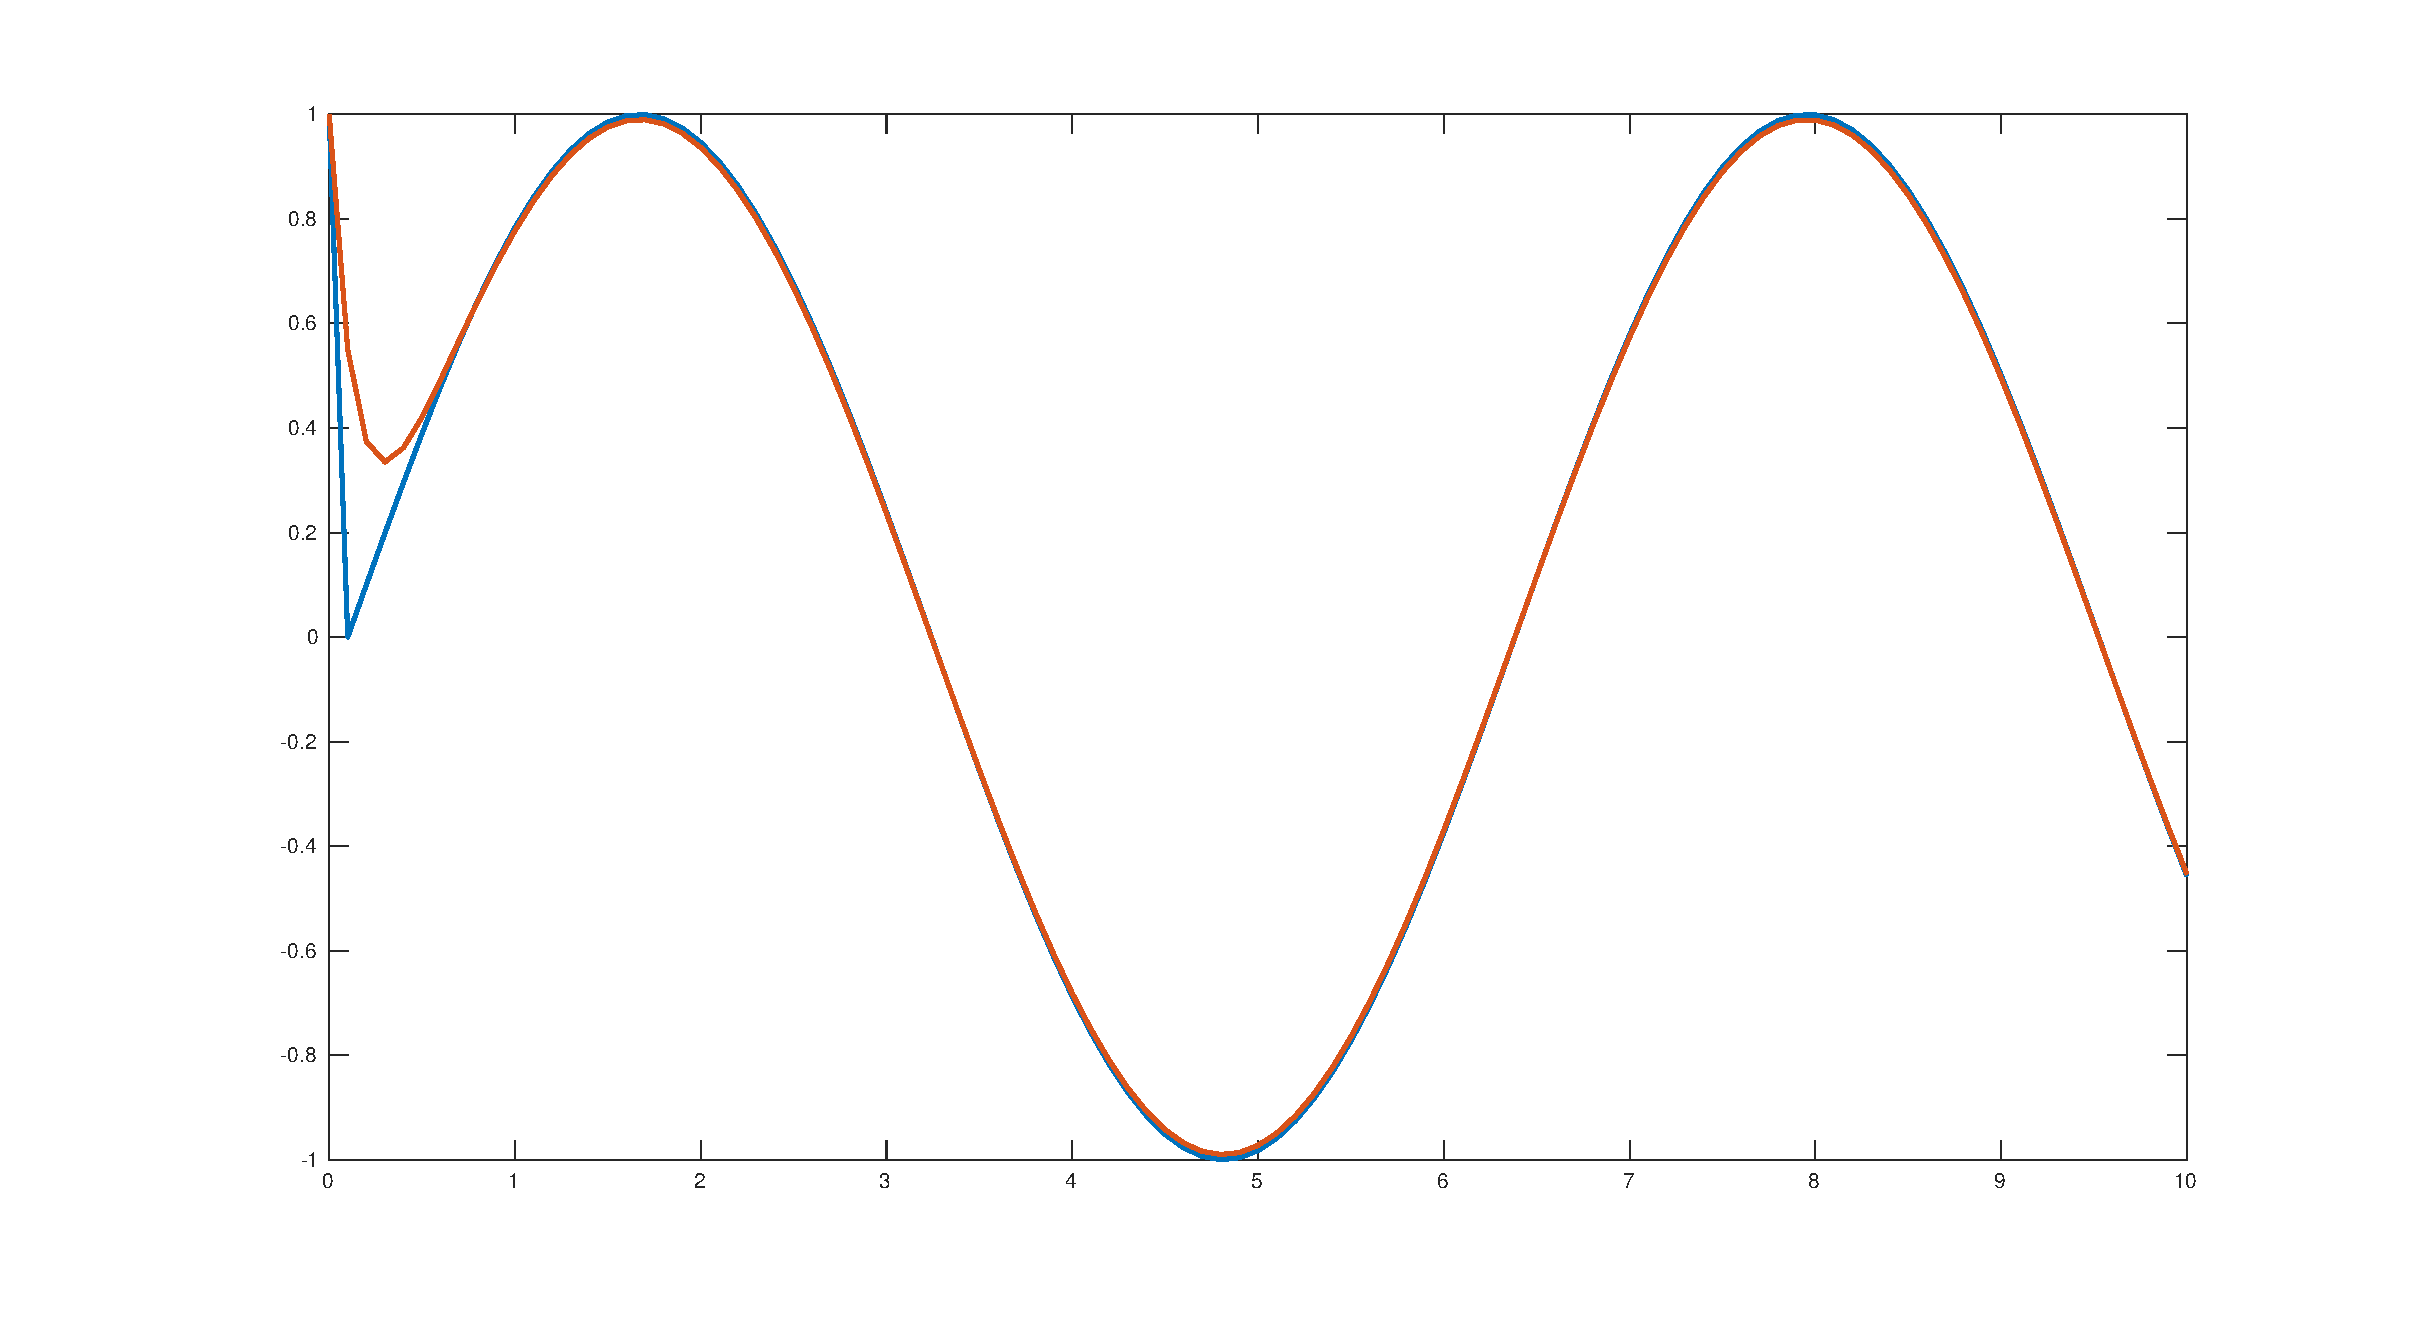
\includegraphics[width=0.85\textwidth]{./euler.eps}
\end{center}

\section{M\'etodos num\'ericos para PVI con funciones propias de \octave}

\octave tiene dos funciones base para el c\'alculo de soluciones num\'ericas de P.V.I. esta son \texttt{ode23} y \texttt{ode45}.

La funci\'on \texttt{ode45} opera bien con la mayor\'ia de los problemas de EDO y en general debe ser la primera elecci\'on de funci\'on para resolver una EDO. Esta funci\'on es una implementaci\'on de una variaci\'on de los m\'etodos de Runge Kuta.

Las EDO  del tipo \emph{stiff} resultan dif\'iciles de resolver num\'ericamente mediante m\'etodos expl\'icitos. En la pr\'actica, se puede identificar si un problema es \emph{stiff} o no \emph{stiff} utilizando una funci\'on para problemas no \emph{stiff}, como \texttt{ode45}, y viendo si esta es incapaz de converger a una soluci\'on o si los c\'alculos son extremadamente lentos.

Ciertos par\'ametros se pueden controlar para las funciones \texttt{ode23} y \texttt{ode45} usando la funci\'on \texttt{odeset}, algunas de estas son

\begin{center}
    \begin{tabular}{|c||c|p{0.5\textwidth}}
    InitialStep
         &  Primer paso de la malla & Obligar a que el primer paso de la malla construida sea un valor fijo.\\
    MaxStep
        & Tama\~{n}o de paso m\'aximo   & Obligar que las distancias entre nodos consecutivos de una malla sea menor que cierto valor.\\
    RelTol
        & Tolerancia del error relativo & Obligar que el error de cada problema local sea menor que cierto valor.\\
    AbsTol
         & Tolerancia del error absoluto    & Obligar que el mayor error local sea menor que cierto valor.  \\
    \end{tabular}
\end{center}

Por ejemplo, el \href{ftp://ftp.ing-mat.udec.cl/pub/ing-mat/asignaturas/521230/ejercicios/2018-2/P3.m}{programa}

\begin{lstlisting}
fvdp = @(t,y) [exp(-0.05*t)*cos(t)];
opt = odeset ("OutputFcn", @odeplot, "RelTol", 1e-10);
sol = ode45 (fvdp, [0 50*pi], [2], opt);
\end{lstlisting}
resuelve usando la funci\'on \texttt{ode45} el P.V.I.
$$
\begin{array}{cl|}
y'(t) &=e^{-0.05\,t} cos(t) \\
y(0)    &=2\\ \hline
\end{array}
$$
con un error relativo menor a $10^{-10}$, muestra el resultado mediante una animaci\'on de los c\'alculos de cada nodo de la soluci\'on num\'erica. y graba las im\'agenes de la soluci\'on num\'erica en la variable \texttt{sol}.

\section{Ejemplos de uso de los \emph{solver} num\'ericos de \octave}
A continuaci\'on introducimos diversos fen\'omenos que se pueden modelar mediante un PVI y ejemplificamos el uso de las funciones que \octave posee para aproximar su soluci\'on.

\subsection{Carga de un circuito RC}
Un circuito RC es diagramado seg\'un 
\begin{center}
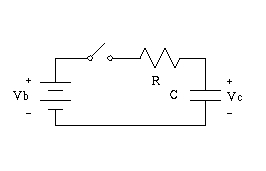
\includegraphics[width=0.5\textwidth]{cap1.jpg}
\end{center}
La carga del capacitor de este circuito depende de la diferencia de potencial el\'ectrico $V_{e}$ entregada por la fuente, la resistencia medida en Ohms $[\Omega]$ y la capacidad el\'ectrica del capacitor medida en Faradios $[\mu F]$. Este fen\'omeno es modelado por la ley de Kirchoff en el PVI
$$
\begin{array}{rl|}
C \frac{d}{dt}q(t)+\frac{q(t)}{R} & = V_{e}(t),\\
q(0) & =q_0.\\ \hline
\end{array}
$$
Las siguientes instrucciones de \octave aproximan la soluci\'on de este problema
\begin{lstlisting}
%DATOS
V0=12;		%Voltaje de la fuente
R=1.5*10^(3);	%Resistencia electrica
C=4*10^(-3); 	%Capacidad del capacitor
tf=120;		%Tiempo final 
f=@(t,x) V0/C-x/(R*C); %Funcion del modelo

tiempo=[0 tf]; 	%intervalo de tiempo
q0=0;		%Carga inicial
[t,q]=ode45(f,tiempo,q0); %Solucion numerica
plot(t,q,'r')
xlabel('t')
ylabel('q');
title('Carga del condensador')
\end{lstlisting}
El gr\'afico generado por este programa es
\begin{center}
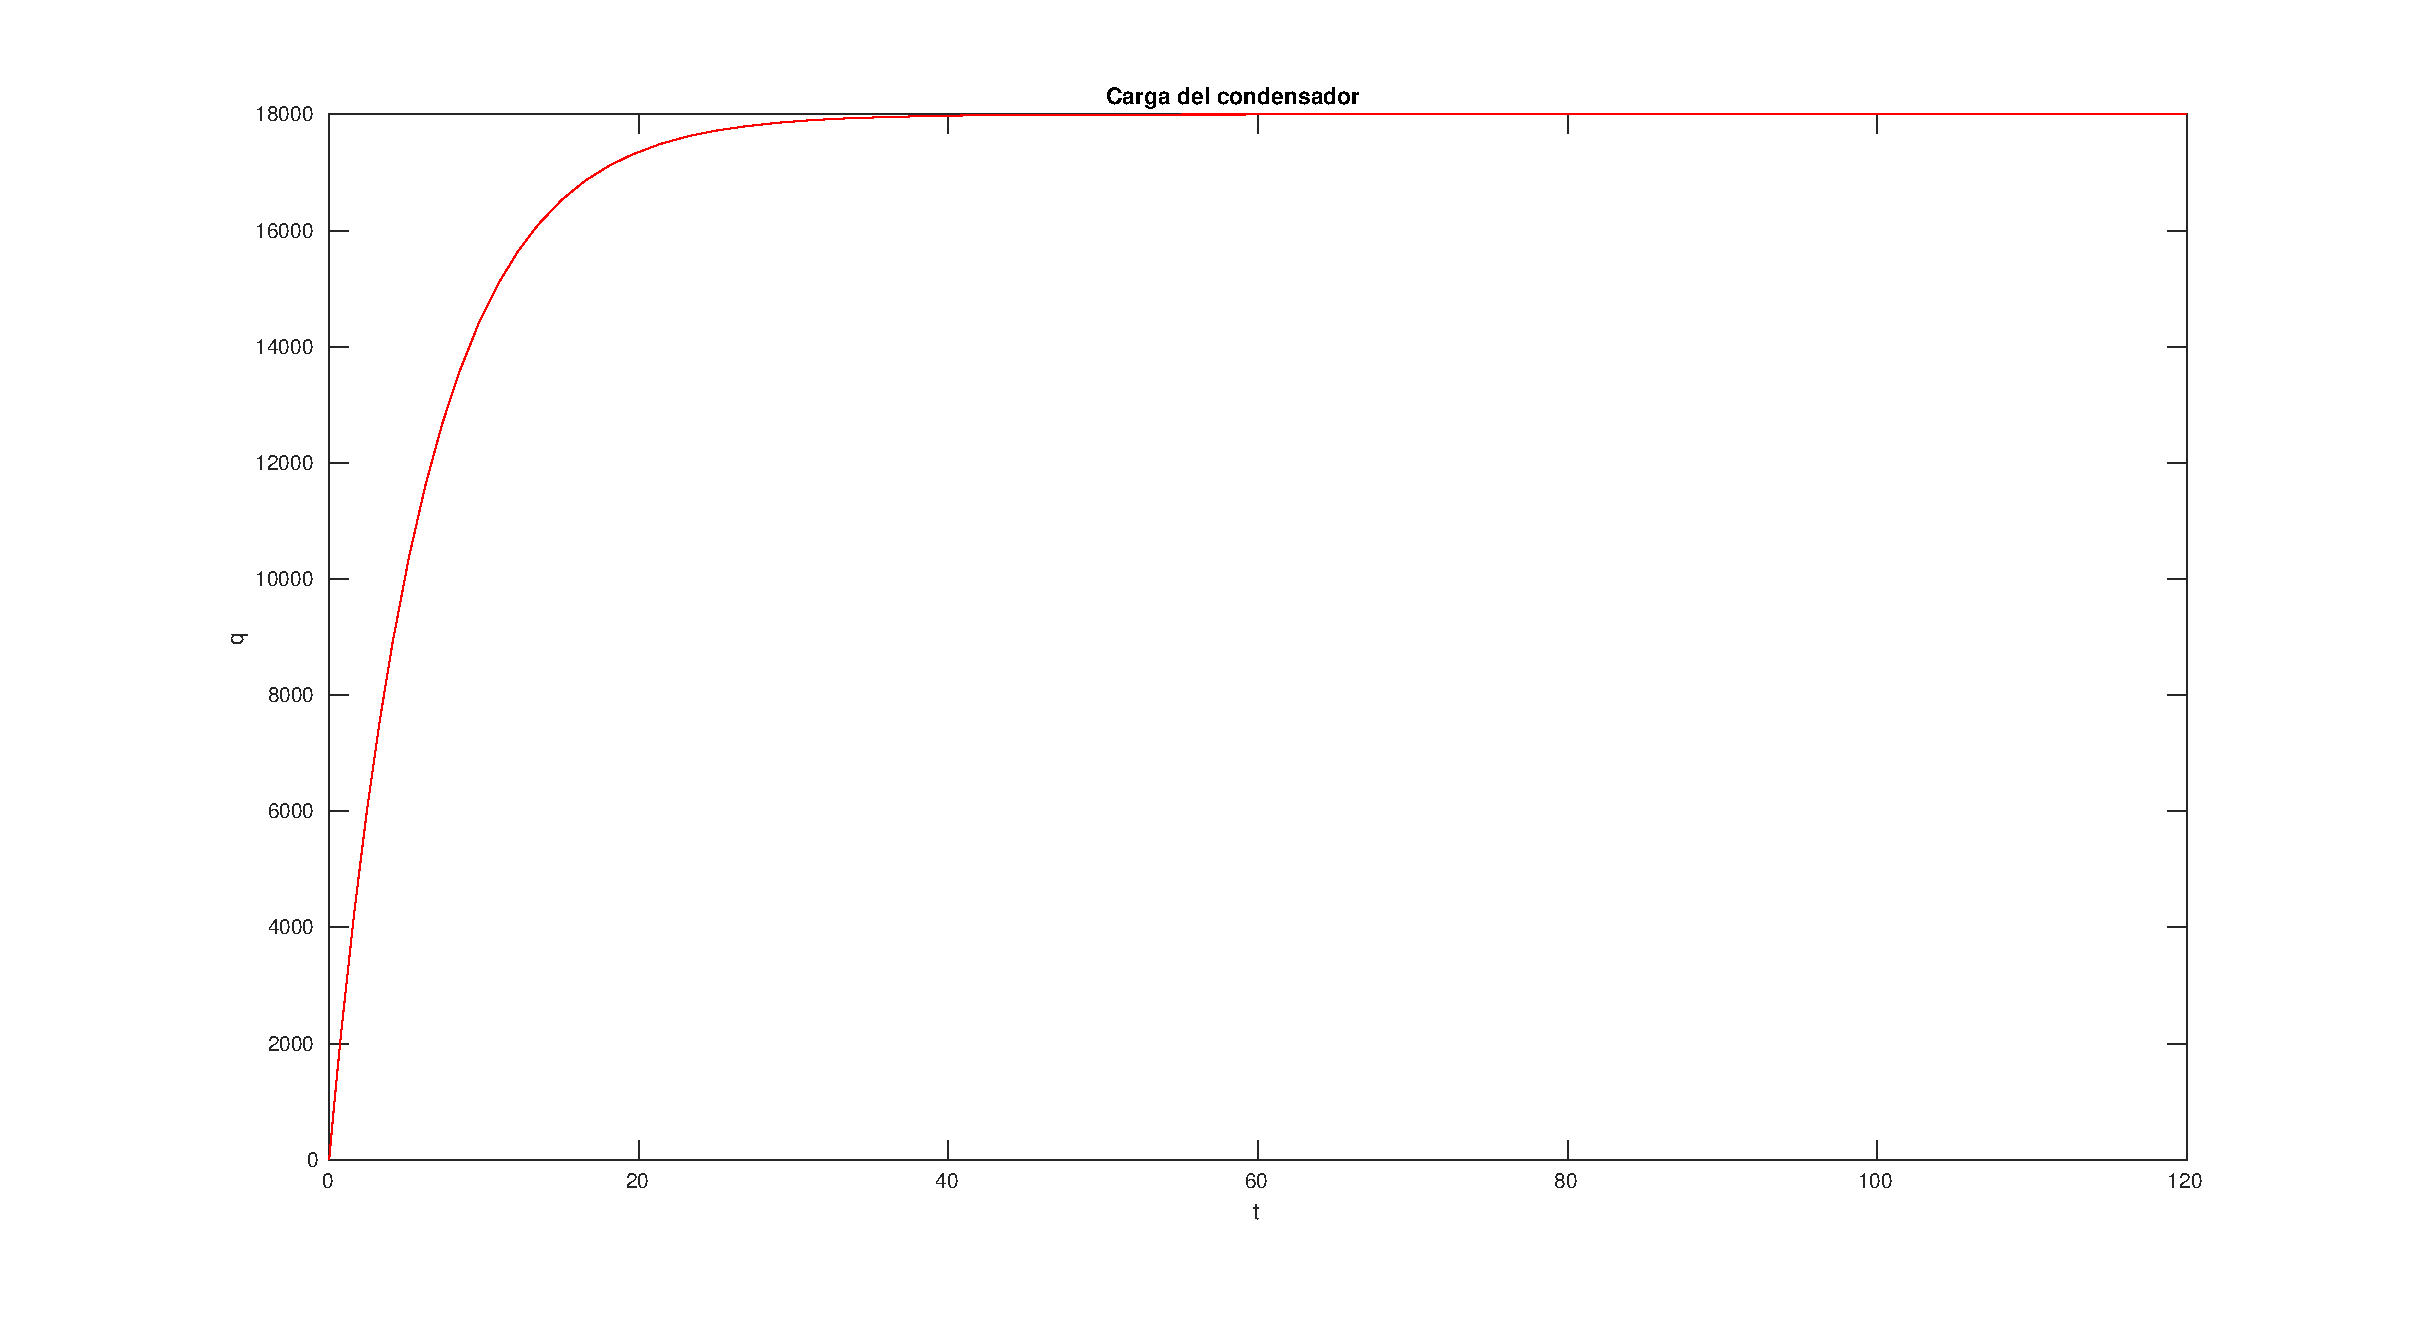
\includegraphics[width=0.85\textwidth]{eje1.eps}
\end{center}

\subsection{Ecuaci\'on de conservaci\'on}
Del balance de masa en un sistema cerrado se deriva la relaci\'on
$$
\left(
\begin{minipage}{0.15\textwidth}
La raz\'on de cambio de $Q(t)$,
\end{minipage}
\right)
=
\left(
\begin{minipage}{0.15\textwidth}
La raz\'on a la que entra $Q(t)$
\end{minipage}
\right)
-
\left(
\begin{minipage}{0.15\textwidth}
La raz\'on a la que sale $Q(t)$
\end{minipage}
\right).
$$
Este principio tiene varias aplicaciones en qu\'imica, f\'isica e ingenier\'ia.

\subsubsection{Disoluci\'on qu\'imica}

En qu\'imica una cantidad se suele medir en unidades de masa como son gramos, kilogramos o en cantidades como los moles. El volumen se puede medir en litros, metros c\'ubicos u otras derivadas. La concentraci\'on de un soluto en un solvente se suele medir en unidades derivadas de estas como $[gr/L]$. El flujo de un solvente se puede medir en unidades de caudal como $[L/s]$ o $[L/h]$.

Un tanque de $1500[L]$ contiene inicialmente $600[L]$ de agua con $1[Kg]$ de sal disuelto en ella. En un momento se le empieza a agregar agua a una raz\'on de $9[L/h]$ con una concentraci\'on de sal de $0.5[g/L]$. Si esta soluci\'on bien mezclada sale del tanque a $6[L/h]$, ?`cu\'anta sal hay en el estanque cuando \'este se llena?

Este problema se modela mediante el PVI
$$
\begin{array}{rl|}
q'(t)	&= 0.5[g/L] \cdot 9[L/h] - \frac{q(t)}{600+3t} [g/h],\\
q(0)	&= 1000[g]. \\ \hline
\end{array}
$$
donde $q(t)$ es la cantidad de sal en el estanque medida en gramos y $t$ es las horas transcurridad desde el inicio de la disoluci\'on.

El siguiente c\'odigo ejemplifica el uso de \texttt{ode45} para la soluci\'on de este problema
\begin{lstlisting}
V0=600; %Volumen inicial
q0=1000;%Sal inicial
Qin=9;  %Caudal de entrada
Qout=6; %Caudal de salida
Cin=0.5;  %Concentracion de entrada
f=@(t,q) Qin*Cin-q/(V0+(Qin-Qout)*t)*Qout;
[t,q]=ode45(f,[0,120],q0);
plot(t,q,'-');
xlabel('tiempo medido en horas');
ylabel('cantidad de sal en el estanque');
title('Cantidad de sal en el estanque');
\end{lstlisting}
El gr\'afico generado por este programa es
\begin{center}
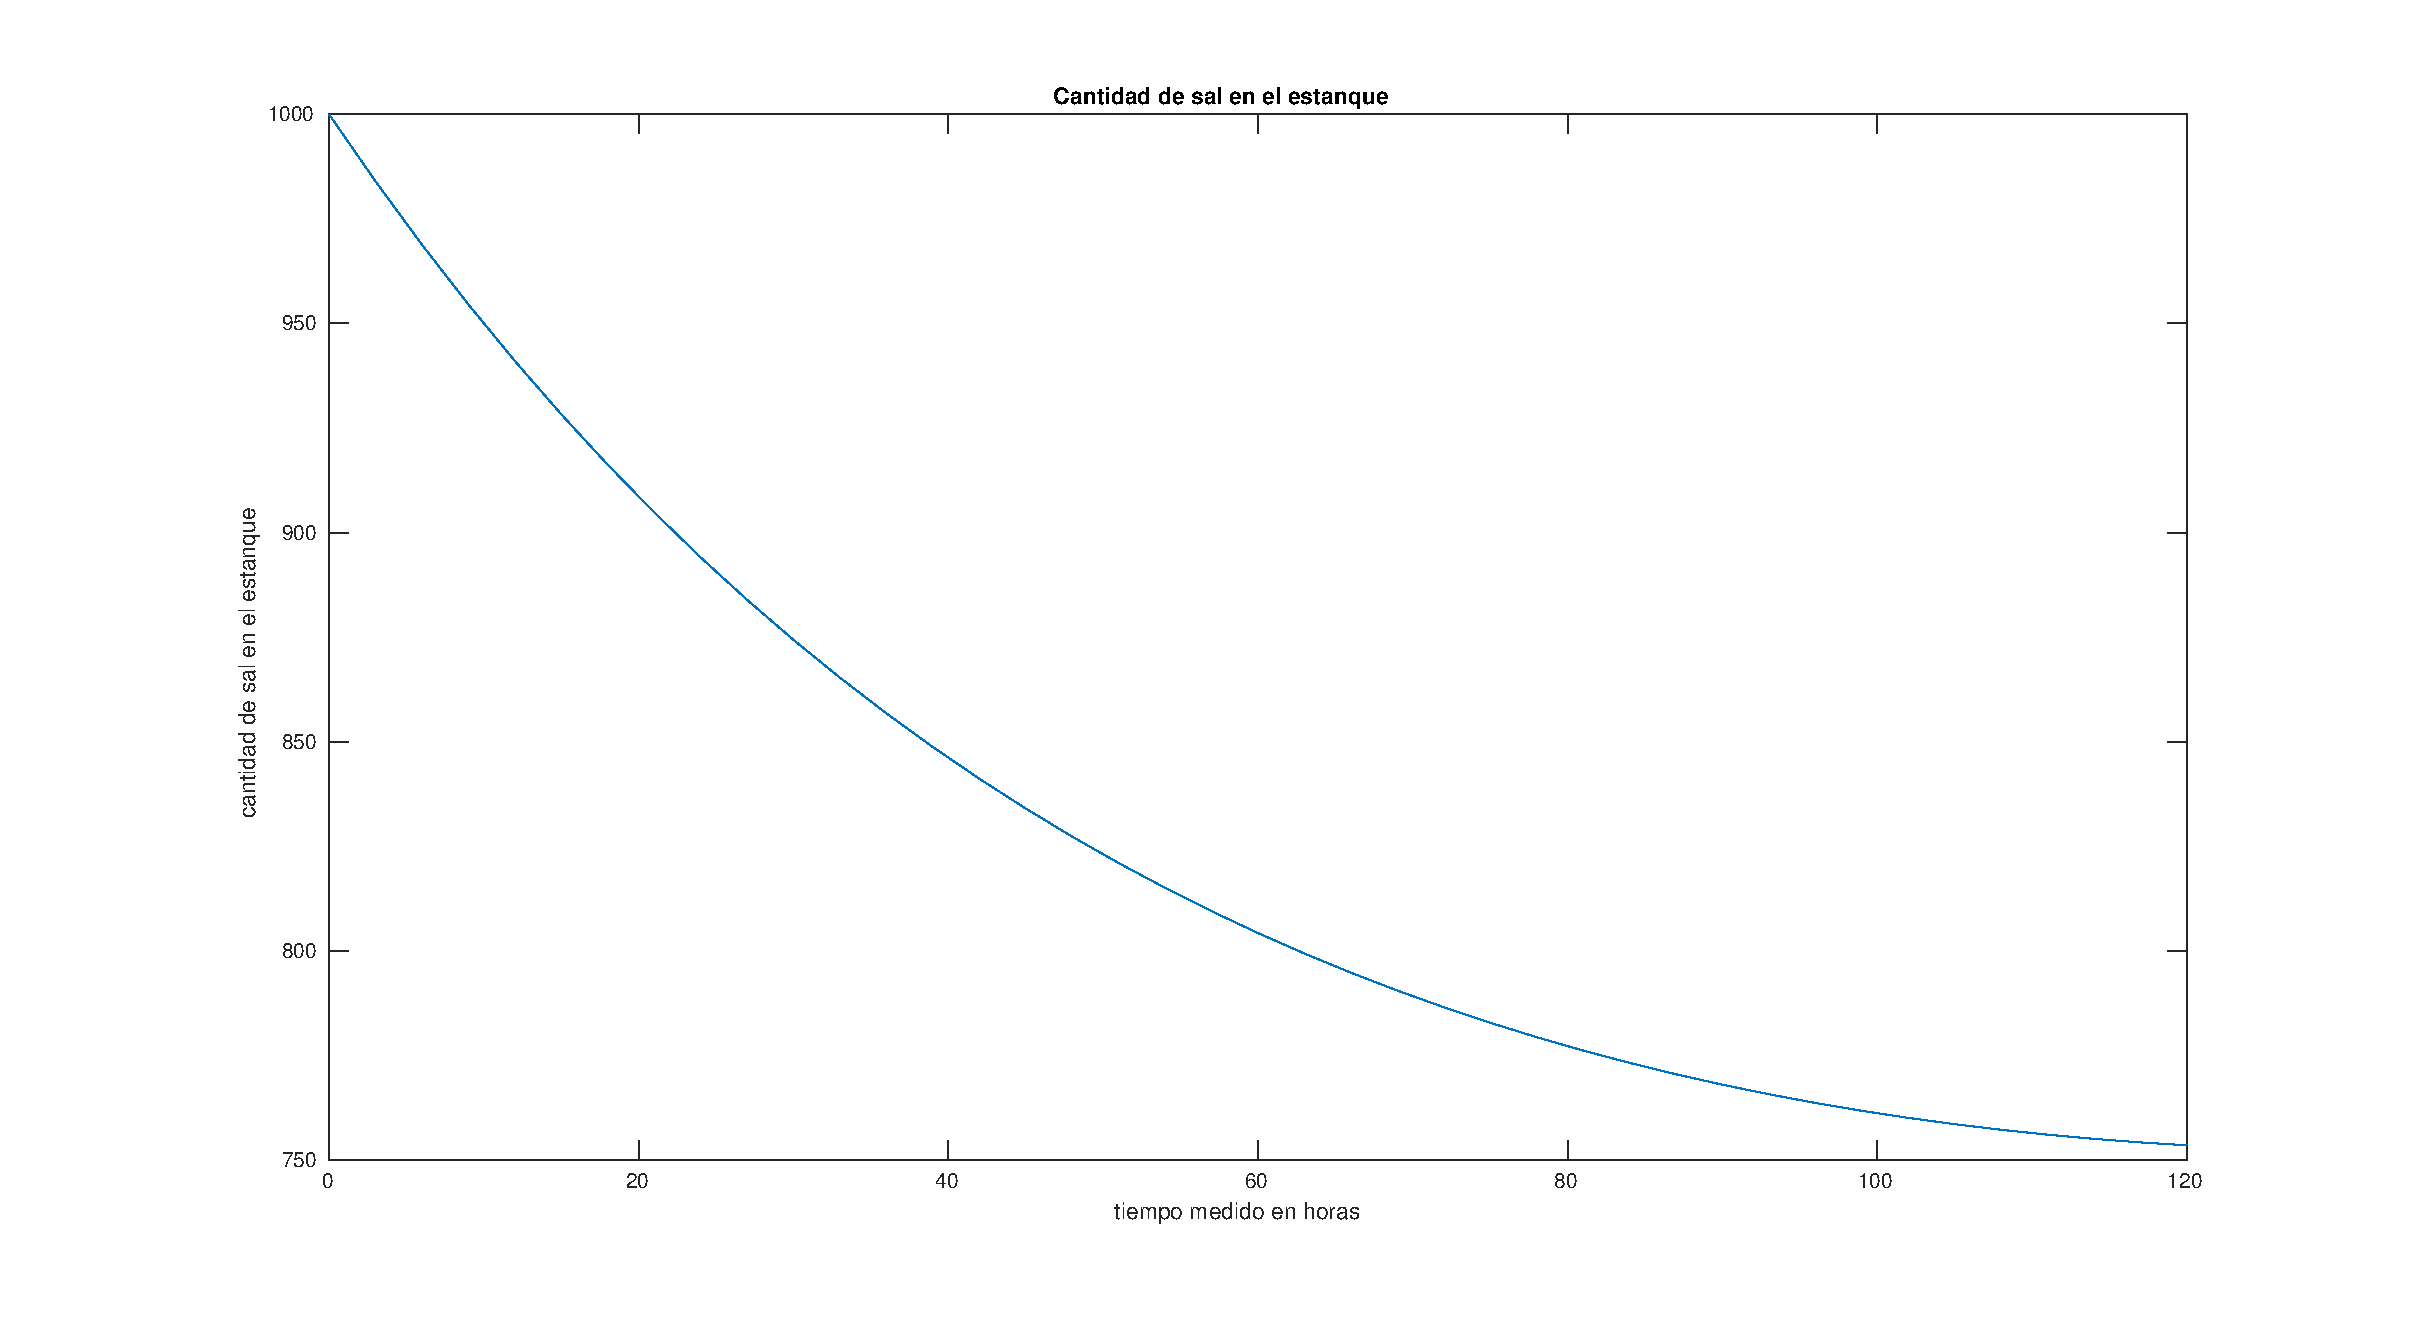
\includegraphics[width=0.85\textwidth]{eje2.eps}
\end{center}

\subsection{Vaciado estanques}
El vaciado de un estanque es un proceso en r\'egimen no estacionario debido a que tenemos una salida de masa de un sistema a una velocidad variable que depender\'a de la altura del fluido en el estanque. Sin embargo, mediante el balance de energ\'ia para una part\'icula de masa $m$ en el fluido,
$$
\frac{1}{2}mv^2=mgh \implies v=\sqrt{2gh}.
$$
La \'ultima ecuaci\'on es conocida en hidrodin\'amica como la ley de Torricelli y establece la velocidad o flujo de salida $v$ de un estanque a trav\'es de un agujero que est\'a a una profundidad $h$. En la pr\'actica esta ley no considera la presencia de fuerzas disipativas, lo que motiva a corregir esta relaci\'on en la forma
$$
v=c\sqrt{2gh},
$$
donde $c \in [0,1]$ se llama \emph{coeficiente de descarga}.

Supongamos que un estanque cil\'indrico para combustible de $5[m]$ de altura y $1000[L]$ de capacidad se encuentra lleno. Desde un momento se le hace una perforaci\'on circular de diametro $2[mm]$ en un cara inferior, por donde empieza a escurrir petr\'oleo. 

Este problema se modela mediante el PVI
$$
\begin{array}{rl|}
\frac{1}{5}h'(t)	&= -\pi r^2\cdot \sqrt{2 g h(t)},\\
h(0)	&= 5[m], \\ \hline
\end{array}
$$
donde $h(t)$ es la altura de la columna de petr\'oleo en el estanque en funci\'on del tiempo $t$ medido en segundos, $r$ es el radio de la perforaci\'on y $g$ es la aceleraci\'on de gravedad.

El siguiente c\'odigo ejemplifica el uso de \texttt{ode45} para la soluci\'on de este problema
\begin{lstlisting}
Ab=1/5; %Superficie de la base del estanque
Vtot=1; %Volumen total del estanque
r=0.002; %Radio de la perforacion
g=9.81;  %Aceleracion de gravedad
dh=@(t,h) -Ab/Vtot*pi*r^2*sqrt(2*g*h);
[t,h]=ode45(dh,[0,60*60*24*3],5);
plot(t,h)
xlabel('tiempo medido en s');
ylabel('altura en el estanque');
title('Vaciado de un estanque');
\end{lstlisting}
\begin{center}
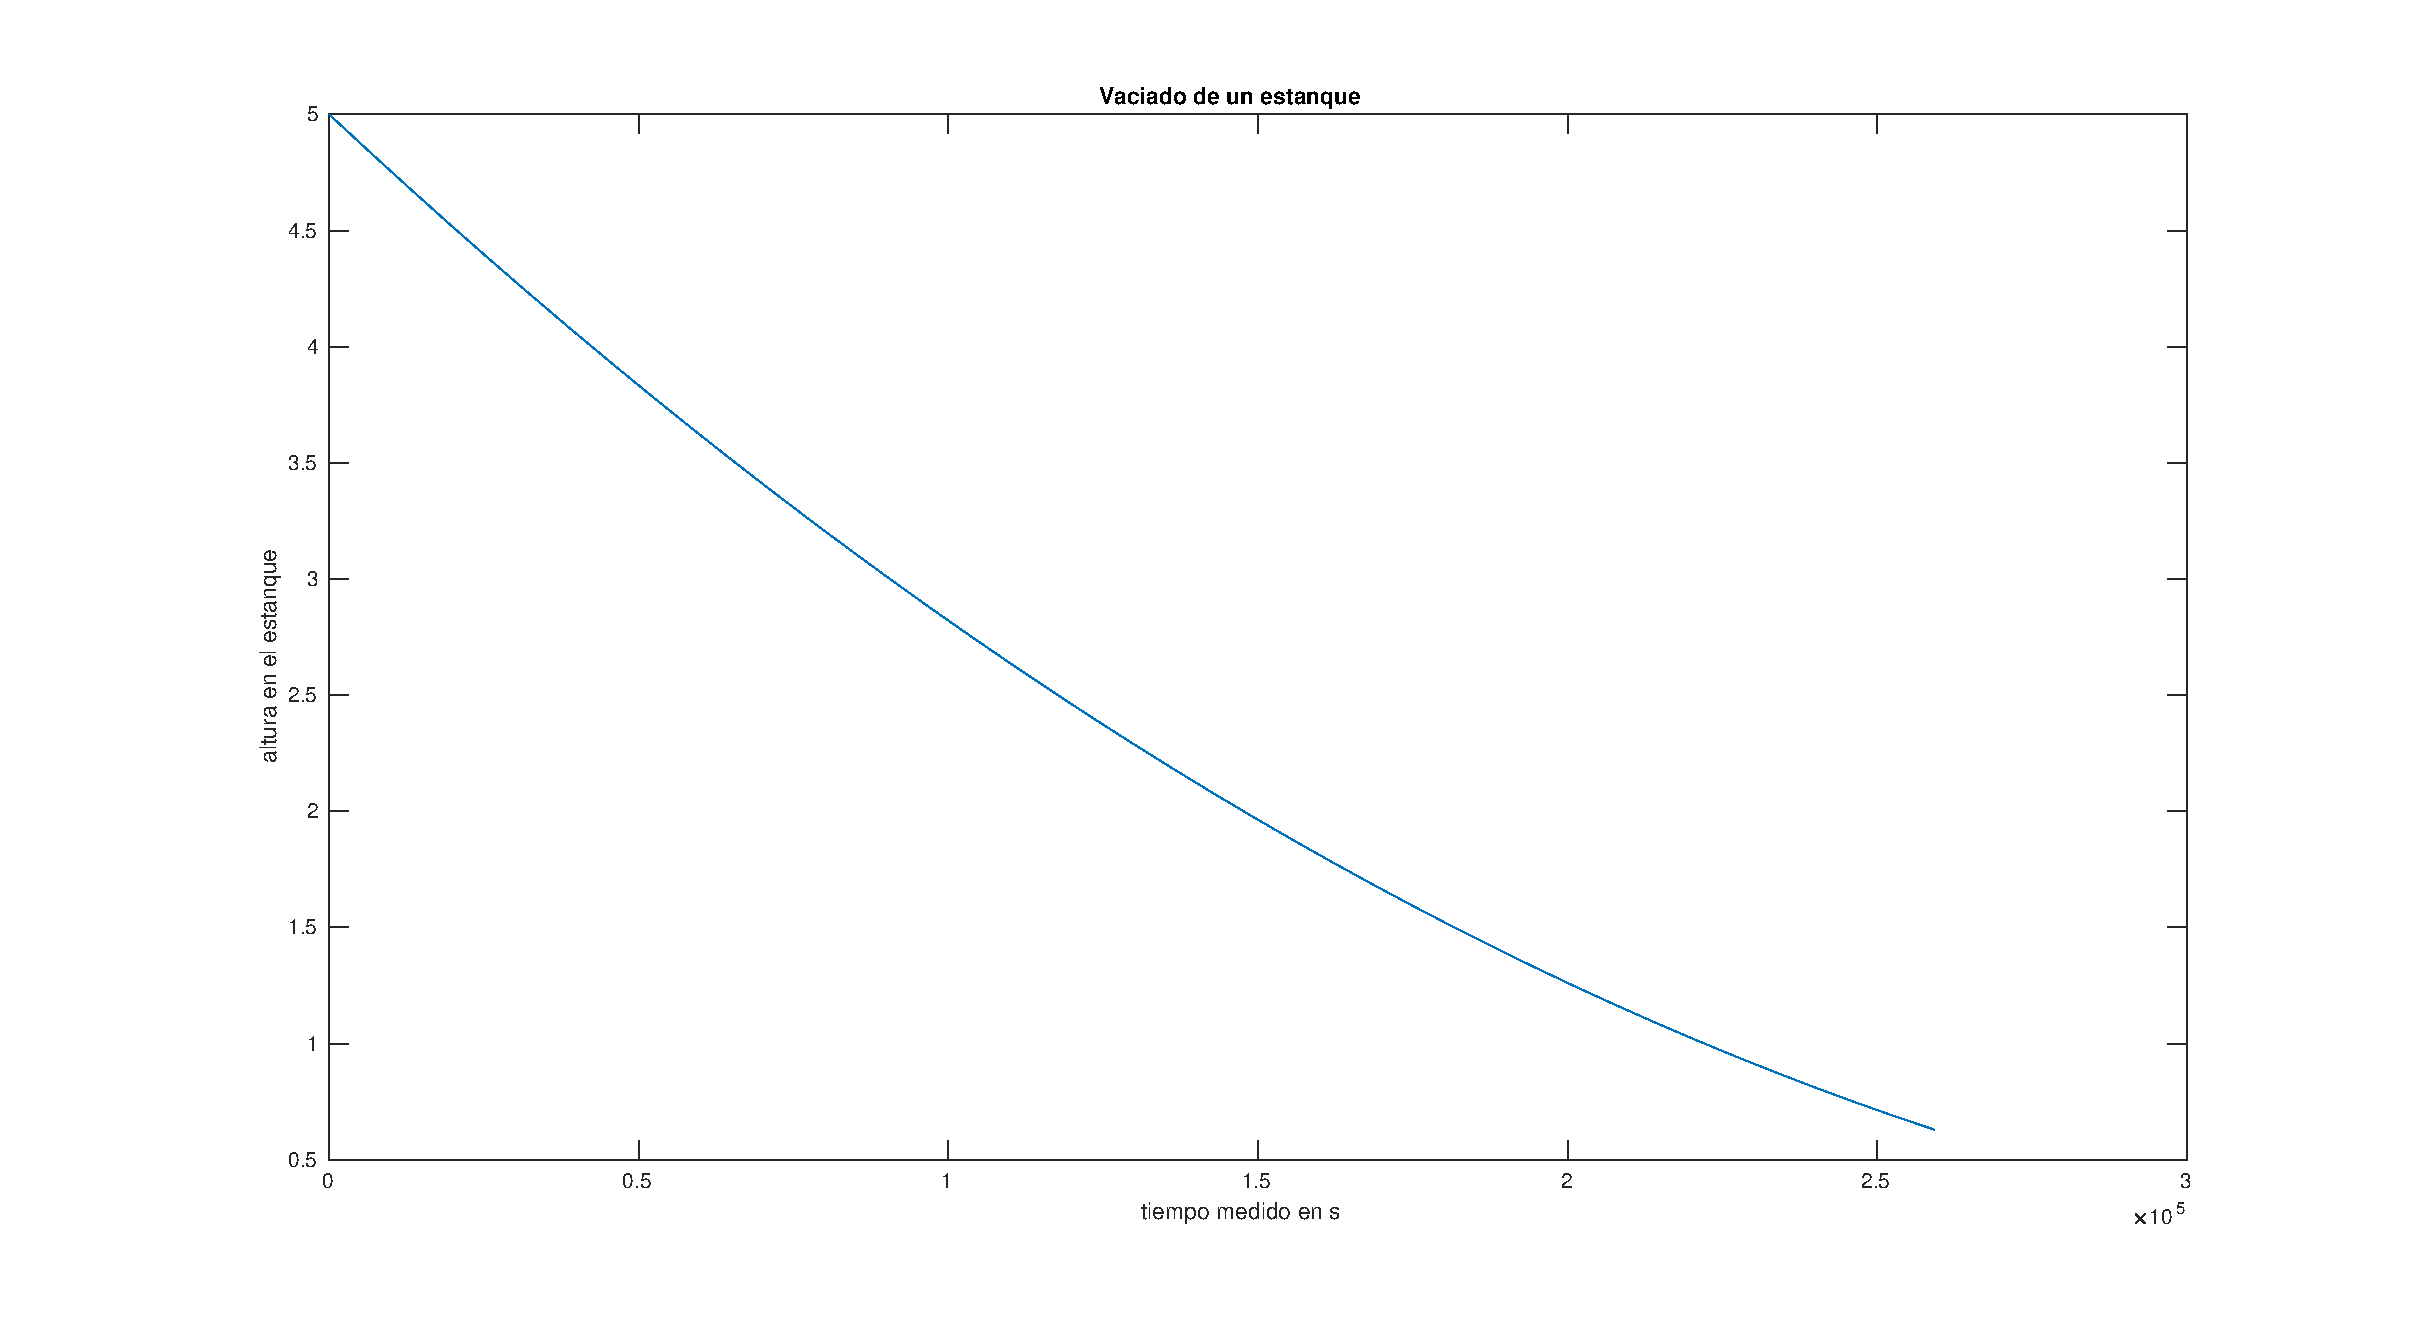
\includegraphics[width=0.85\textwidth]{eje3.eps}
\end{center}

\subsection{Sistemas de ecuaciones diferenciales}

Un PVI de orden $n$
$$
\left\{
\begin{array}{l}
y^{(n)}=f\left(x,y,y',\ldots,y^{(n-1)}\right), \qquad x\in[a,b],\\
y(a)=z_{01},\,y'(a)=z_{02},\ldots,\,y^{n-1}(a)=z_{0n},
\end{array}
\right.
$$
se puede expresar como un sistema de $n$ ecuaciones de primer orden al definir:
$$
\boldsymbol{z}=
\left(
\begin{array}{c}
z_1\\
z_2\\
\vdots\\
z_n
\end{array}
\right)
=\left(
\begin{array}{c}
y\\
y'\\
\vdots\\
y^{(n-1)}
\end{array}
\right).
$$
En efecto,
$$
\boldsymbol{z}'=
\left(
\begin{array}{c}
z_1'\\
z_2'\\
\vdots\\
z_n'
\end{array}
\right)
=\left(
\begin{array}{c}
y'\\
y''\\
\vdots\\
y^{(n)}
\end{array}
\right)
=\left(
\begin{array}{c}
z_2\\
z_3\\
\vdots\\
f(x,z_1,z_2,\ldots,z_n)
\end{array}
\right)=: \boldsymbol{f}(x,\boldsymbol{z}).
$$
Adem\'as, las condiciones iniciales quedan:
$$
\boldsymbol{z}(a)=
\left(
\begin{array}{c}
z_1(a)\\
z_2(a)\\
\vdots\\
z_n(a)
\end{array}
\right)
=\left(
\begin{array}{c}
y(a)\\
y'(a)\\
\vdots\\
y^{(n-1)}(a)
\end{array}
\right)
=\left(
\begin{array}{c}
z_{01}\\
z_{02}\\
\vdots\\
z_{0n}
\end{array}
\right)=\boldsymbol{z}_0.
$$
Luego, el PVI
$$
\left\{
\begin{array}{l}
\boldsymbol{z}'=\boldsymbol{f}(x,\boldsymbol{z}),\qquad x\in[a,b],\\
\boldsymbol{z}(a)=\boldsymbol{z}_0,
\end{array}
\right.
$$
es un sistema de EDO de primer orden, al que se pueden aplicar los m\'etodos y comandos antes vistos.

Por el mismo procedimiento, un sistema de ecuaciones diferenciales de orden superior tambi\'en puede expresarse mediante un sistema de EDO de primer orden.
\medskip


\subsubsection{Modelo de presa-depredador}
Suponga que $R(t)$ modela la cantidad de conejos en una isla y $F(t)$ modela la cantidad de zorros en una isla. Se puede suponer que existen ciertas relaciones entre los cambios en las poblaciones de conejos y zorros que podemos resumir en el sistema
$$
\begin{array}{cl}
R'(t) &= a_1 R(t)- a_2 F(t)R(t),\\
F'(t) &=-a_3 F(t)+ a_4 F(t)R(t),
\end{array}
$$
donde $a_1,a_2,a_3,a_4>0$ son constantes fijas que est\'an relacionadas con la reproducci\'on de los zorros y conejos y c\'omo unos alimentan a los otros.

En este contexto las condiciones iniciales $R(0)$ y $F(0)$ representan las poblaciones iniciales de conejos y zorros en la isla.

El siguiente ejemplo muestra una modelaci\'on para ciertos par\'ametros y condiciones iniciales
\begin{lstlisting}
a1=0.4;
a2=0.37;
a3=0.3;
a4=0.05;
f=@(t,x)[a1*x(1)-a2*x(1)*x(2);-a3*x(2)+a4*x(1)*x(2)];
[t,f]=ode15s(f,[0,100],[3,1])
plot(t,f(:,1),t,f(:,2));
legend('Pob. conejos','Pob. zorros')
\end{lstlisting}
\begin{center}
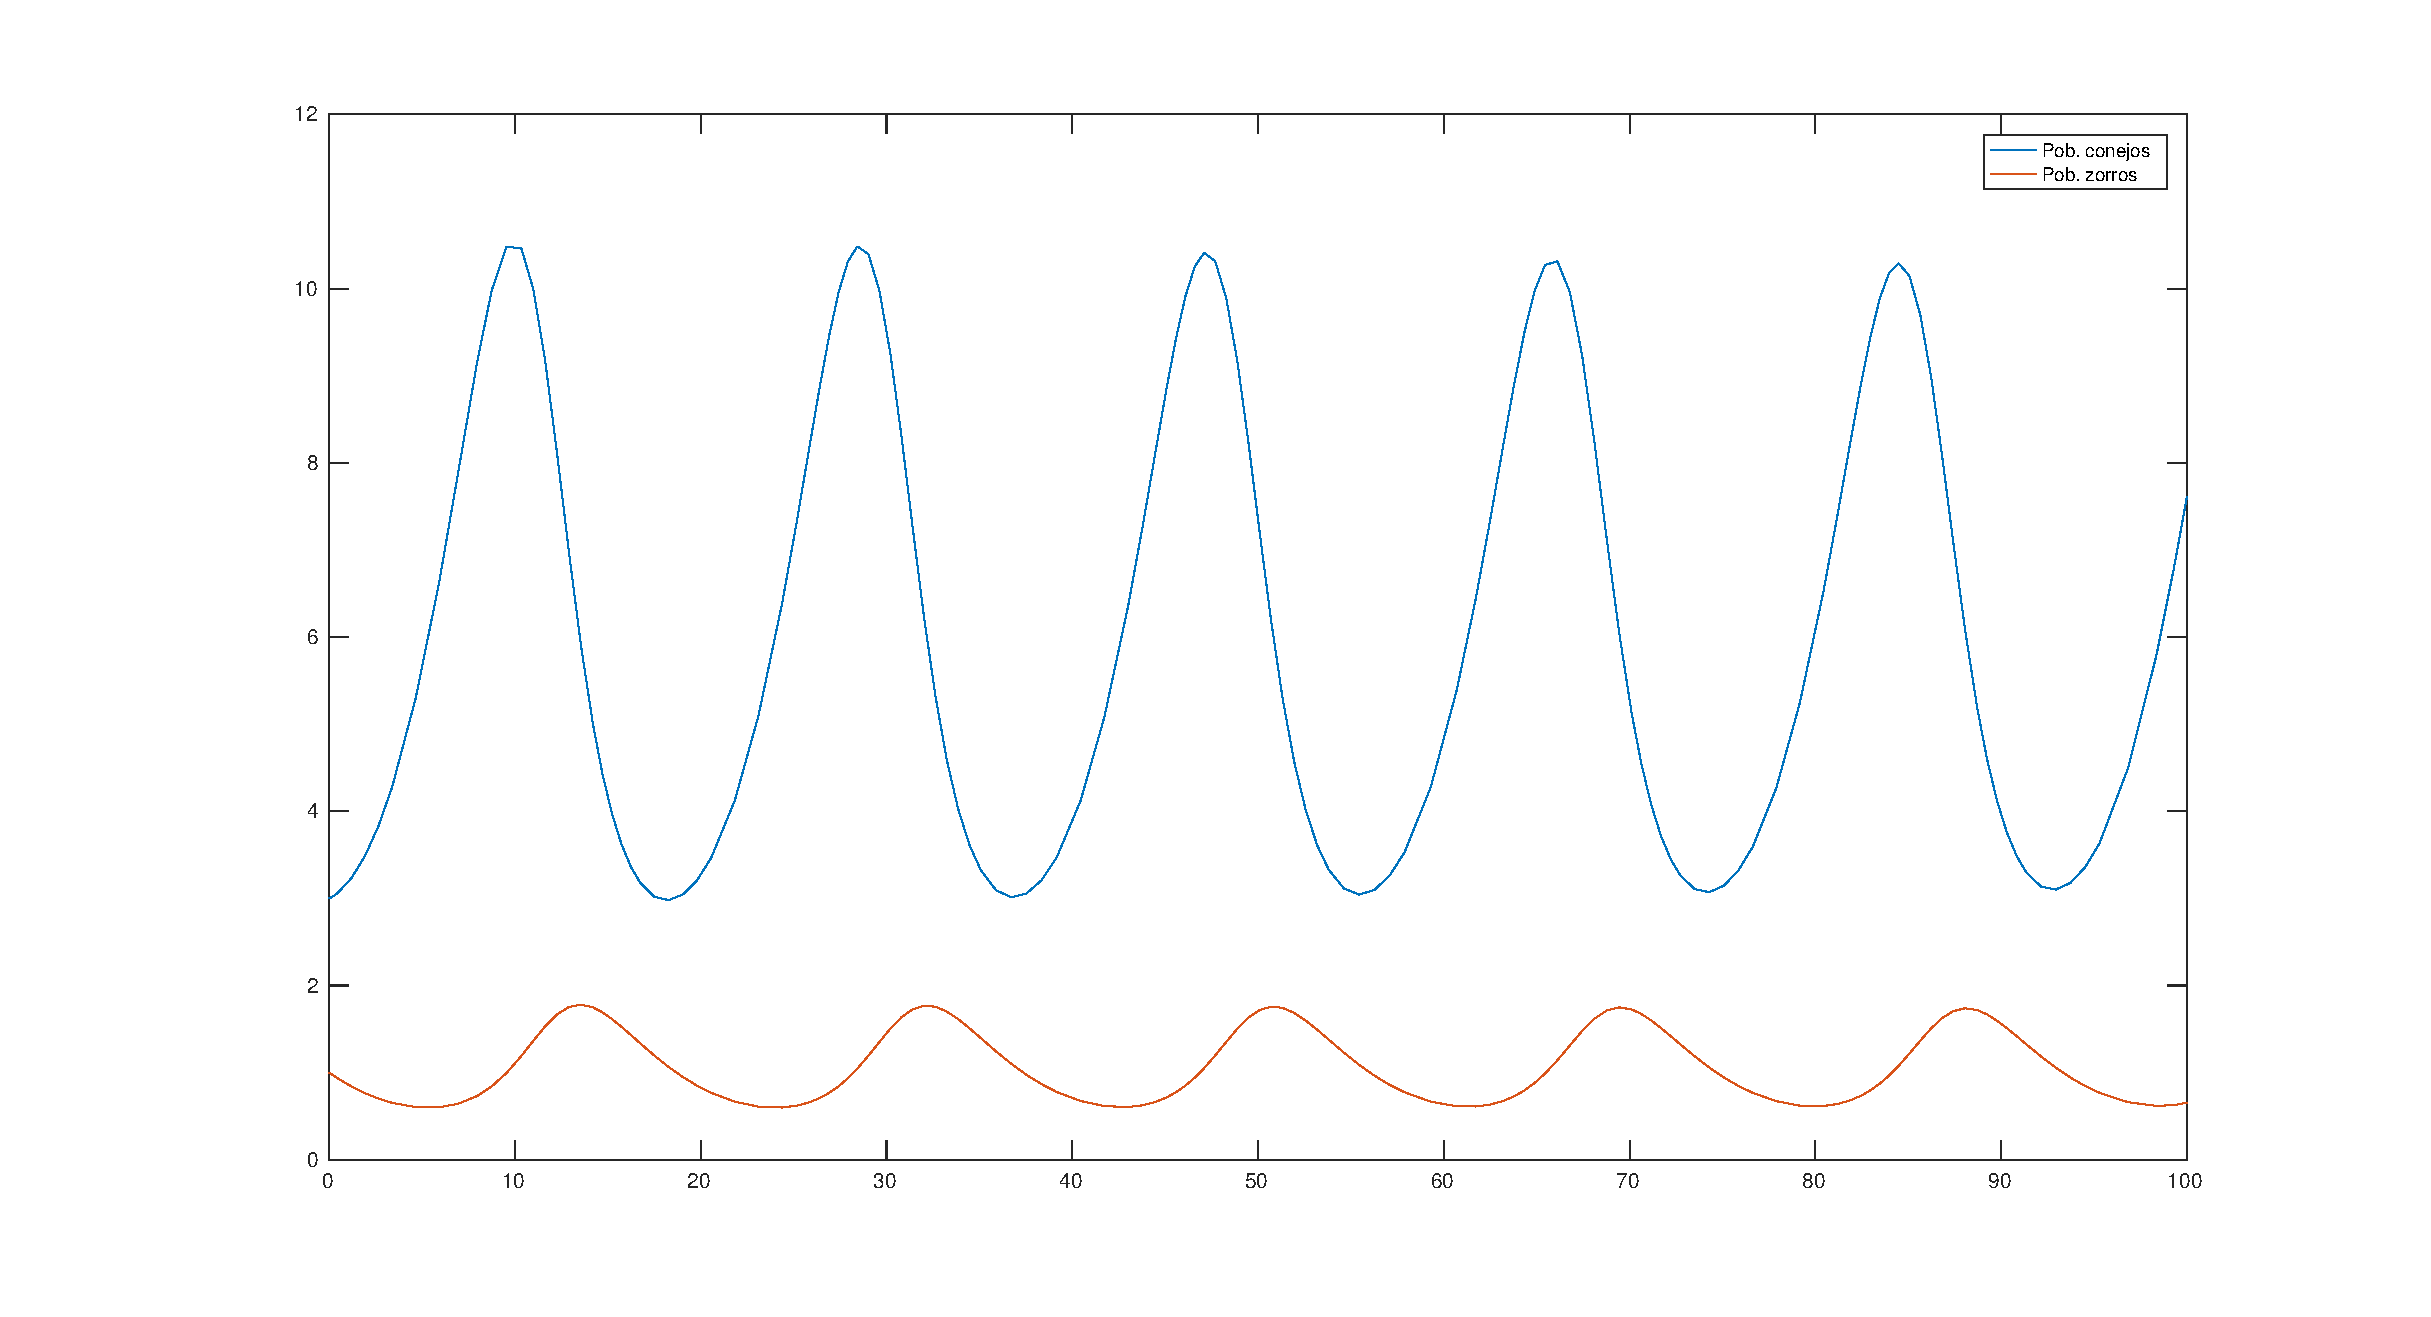
\includegraphics[width=0.85\textwidth]{eje4.eps}
\end{center}

\subsubsection{Sistemas masa-resorte}
El PVI 
$$
\begin{array}{rl|}
mx''(t)+kx(t)'+Rx(t) & = f(t),\\
x(0) & =x_0,\\
x'(0) & =x_1,\\\hline
\end{array}
$$
modela el movimiento de un sistema masa-resorte-amortiguador ideal cuya masa es $m[kg]$, su resorte es de constante $R[N/m]$ y el amortiguador es de coeficiente de difusi\'on $k[N/(m/s)]$.

Este PVI se puede replantear como el sistema de EDO
$$
\begin{array}{rl}
u_1'(t) & =u_2(t),\\
u_2'(t) & =\frac{1}{m} \left( f(t)-ku_2(t)-Ru_1(t)\right),\\
u_1(0) & =x_0,\\
u_2(0) & =x_1,\\ \hline
\end{array}
$$
mediante la sustituci\'on $u_1(t)=x(t)$, $u_2(t)=x'(t)$.  Matricialmente las EDO del sistema se pueden pensar como
$$
\begin{bmatrix}
u_1(t)\\u_2(t)
\end{bmatrix}'
=
\begin{bmatrix}
u_2(t)\\\frac{1}{m} \left( f(t)-ku_2(t)-Ru_1(t)\right).
\end{bmatrix}
$$
Esta es la forma de la funci\'on que se debe ingresar a \octave para resolver el sistema.

El siguiente c\'odigo ejemplifica la modelaci\'on del movimiento de un resorte usando funciones de  \octave.
\begin{lstlisting}
k=1;
r=1;
m=1;
f=@(t,x) [x(2);1/m*(-k*x(2)-r*x(1))];
[t,f]=ode45(f,[0,20],[1,0]);
plot(t,f(:,1),'-k');
xlabel('tiempo');
ylabel('oscilacion');
title('Resorte amortiguado');
\end{lstlisting}
\begin{center}
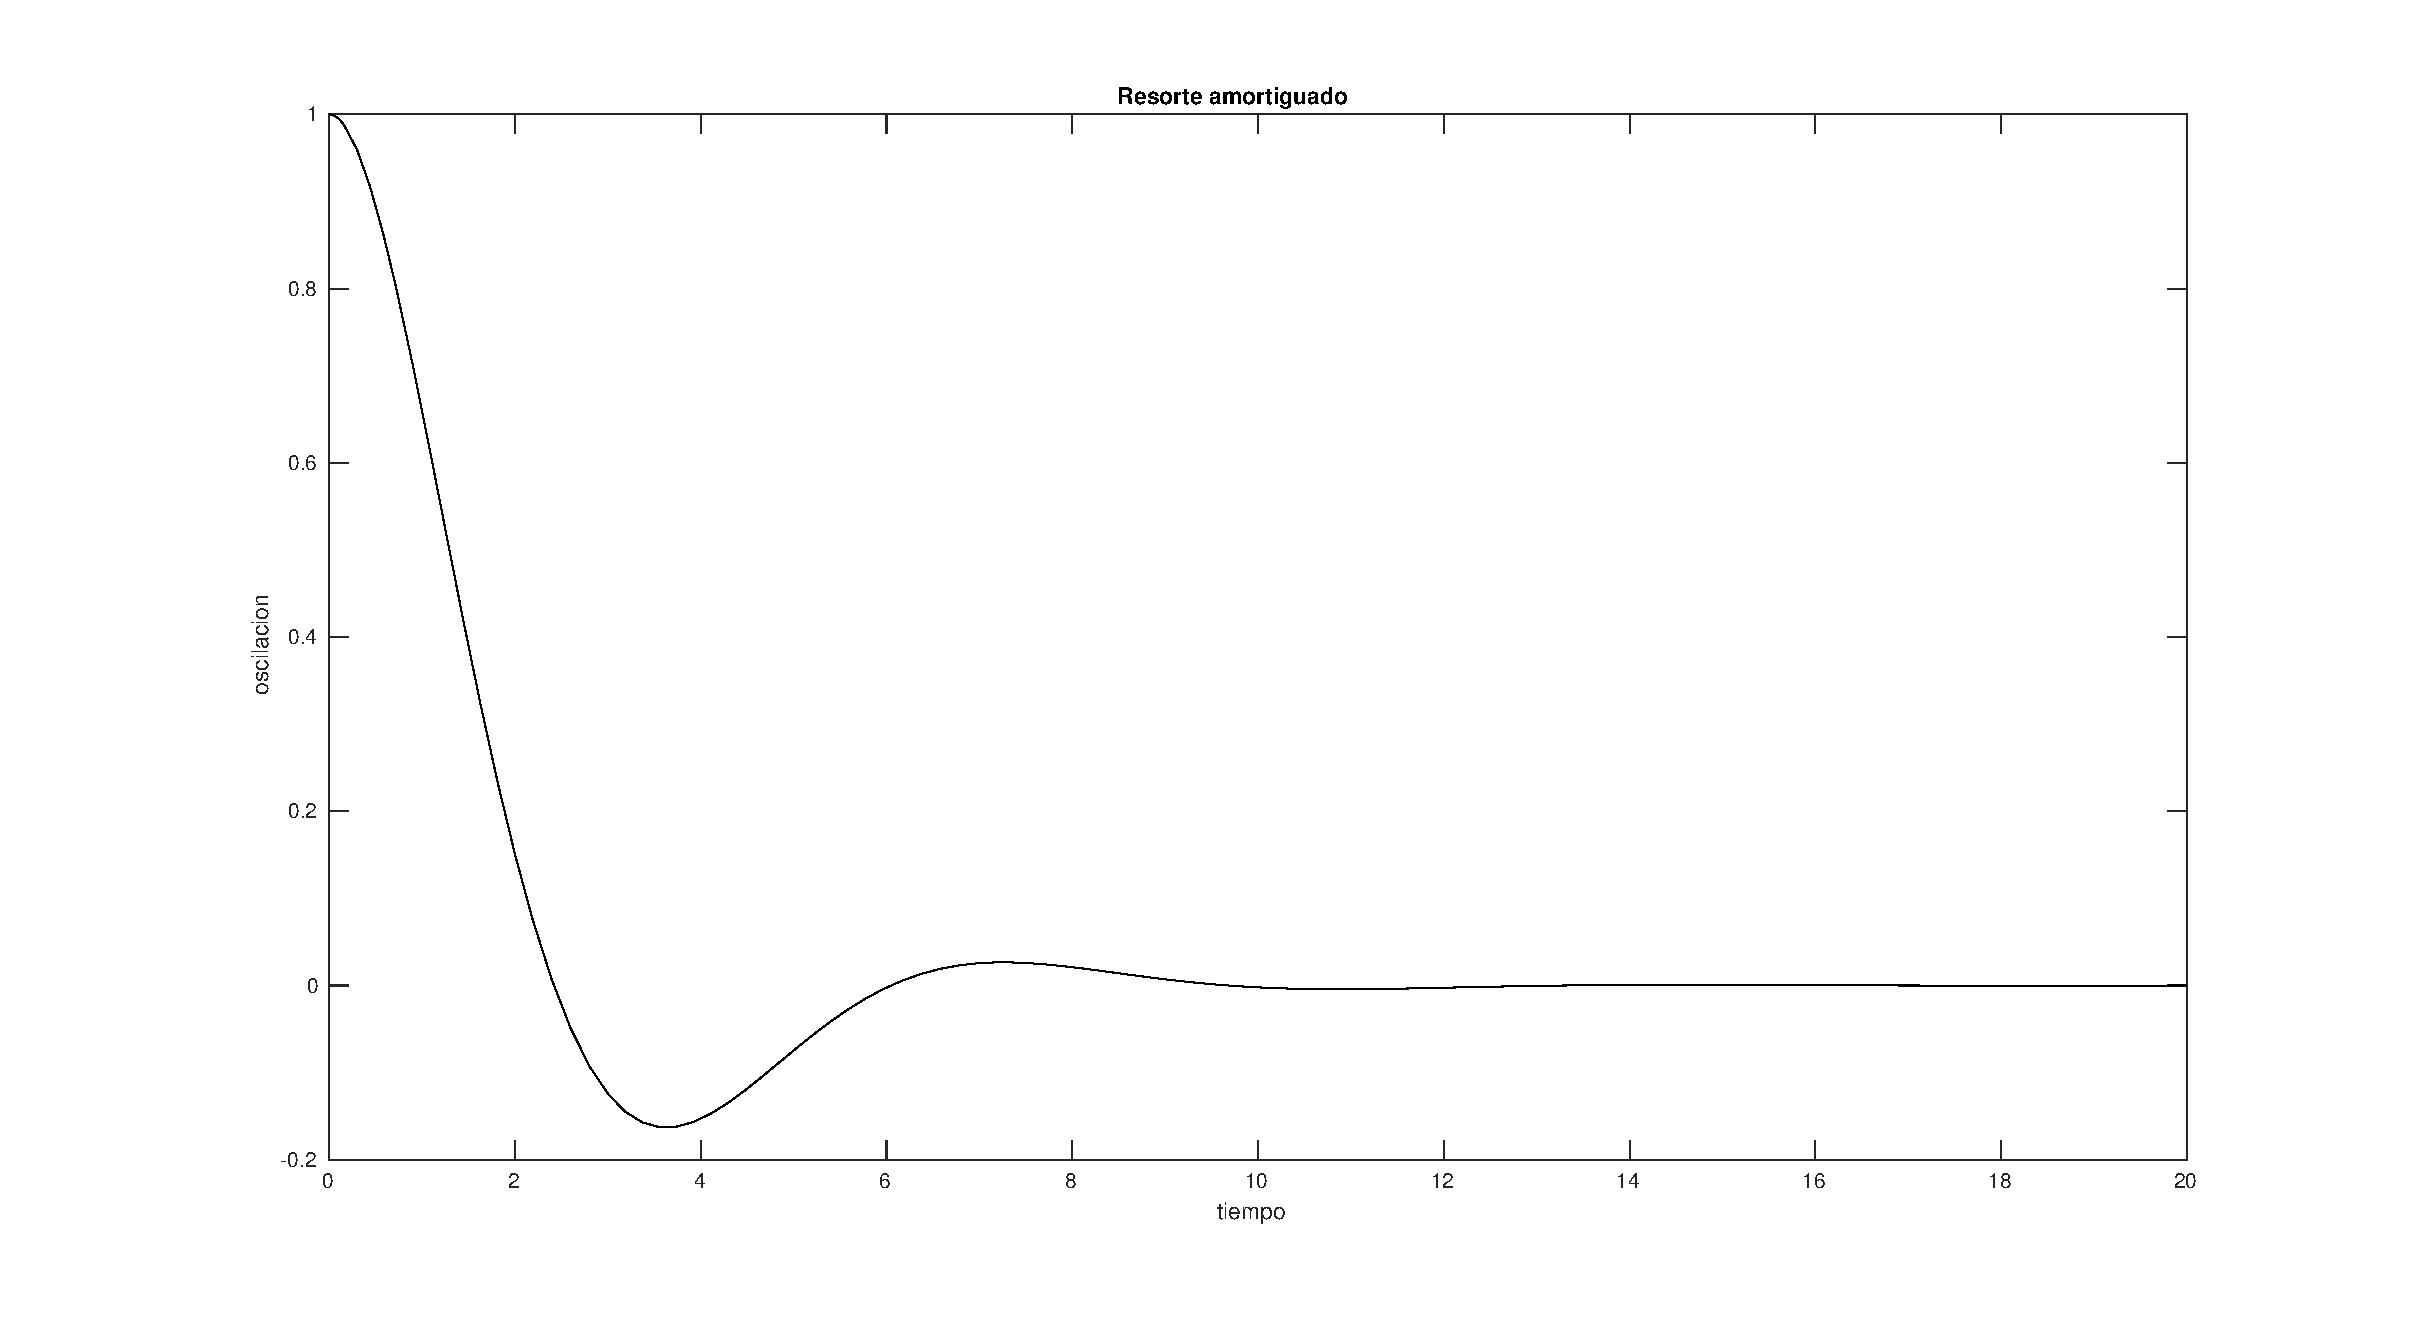
\includegraphics[width=0.85\textwidth]{eje5.eps}
\end{center}

\subsubsection{Circuitos RLC}
Una fuerza electromotriz (por ejemplo, una batería o un alternador) produce un flujo de corriente en un circuito cerrado. Esta corriente provoca una caida de tensi\'on o voltaje en los elementos por inducci\'on, capacidad y resistencia al circular a trav\'es de ellos.
\begin{center}
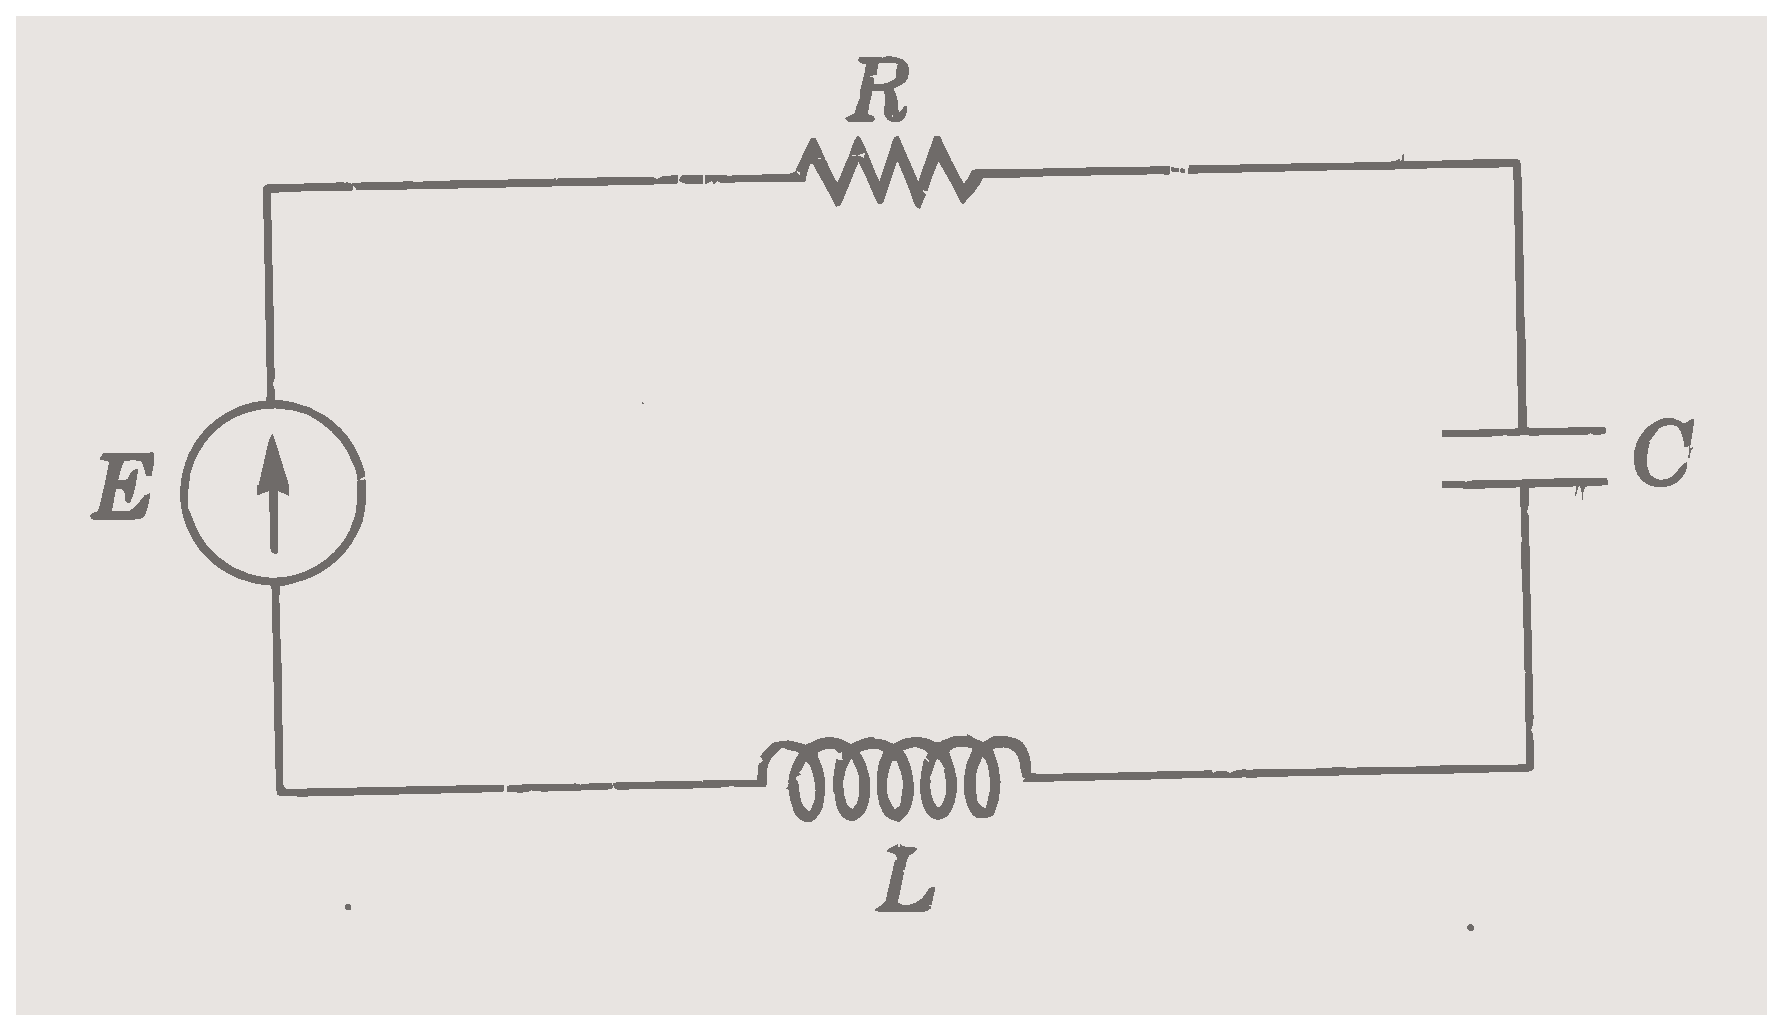
\includegraphics[width=0.5\textwidth]{rlc.eps}
\end{center}
Las leyes b\'asicas, v\'alidas para estos casos y para dicha ca\'ida de tensi\'on son:
\begin{enumerate}
\item En el elemento de resistencia, la ley de Ohm, establece que la resistencia se opone al paso de corriente produciendo una ca\'ida en la fuerza electromotriz proporcional a la intensidad de corriente, seg\'un
$$
E_R=Ri,
$$
donde $R$ es una constante propia de la resistencia e $i$ es la intesidad de corriente.
\item En la bobina o inductancia, esta se opone a cualquier cambio en la corriente, produciendo una ca\'ida en la fuerza electromotriz de magnitud
$$
E_L=L \frac{di}{dt},
$$
donde $L$ es una constante llamado inductancia de la bobina y $t$ es el tiempo.
\item En la capacitancia, capacitor o condensador del circuito se almacena una carga $q$, la carga acumulada se resiste a la entrada de nueva carga, lo que conlleva una ca\'ida de la fuerza electromotriz que viene dada por
$$
E_C=\frac{q}{c},
$$
donde $C$ es una constante propia del capacitor y $q$ es la carga acumulada en el capacitor. Como la corriente es el ritmo de flujo de carga, y por ello el ritmo al que la carga se acumula en el condensador, se tiene que
$$
i=\frac{dq}{dt}
$$
y se puede escribir que
$$
E_C=\frac{1}{C} \int i\,dt
$$
\end{enumerate}
Para formar las E.D.O. que aparecen en este tipo de circuitos el\'ectricos se usa la ley de Kirchhof, la cual establece que
\begin{center}
La suma de las ca\'idas de tensi\'on a lo largo de un circuito cerrado en un sentido fijo es cero.
\end{center}
As\'i, se establece que para el circuito de la figura anterior
$$
L\frac{di}{dt}+Ri+\frac{q}{c} =E
$$
y como $i=\frac{dq}{dt}$, se tiene que
$$
L\frac{d^2q}{dt^2}+R \frac{dq}{dt} + \frac{q}{C}=E
$$
que es una ecuaci\'on diferencial de segundo orden, la cual modela la carga en el circuito o en el capacitor $q$ en funci\'on del tiempo transcurrido.

Usando lo anterior el P.V.I.
$$
\begin{array}{rl|}
0.1 q''(t)+2 q'(t) + 260q(t) &=100 sen(60t),\\
q(0) & =0,\\
q'(0) & =0,\\\hline
\end{array}
$$
modela la carga acumulada en el capacitor del circuito
\begin{center}
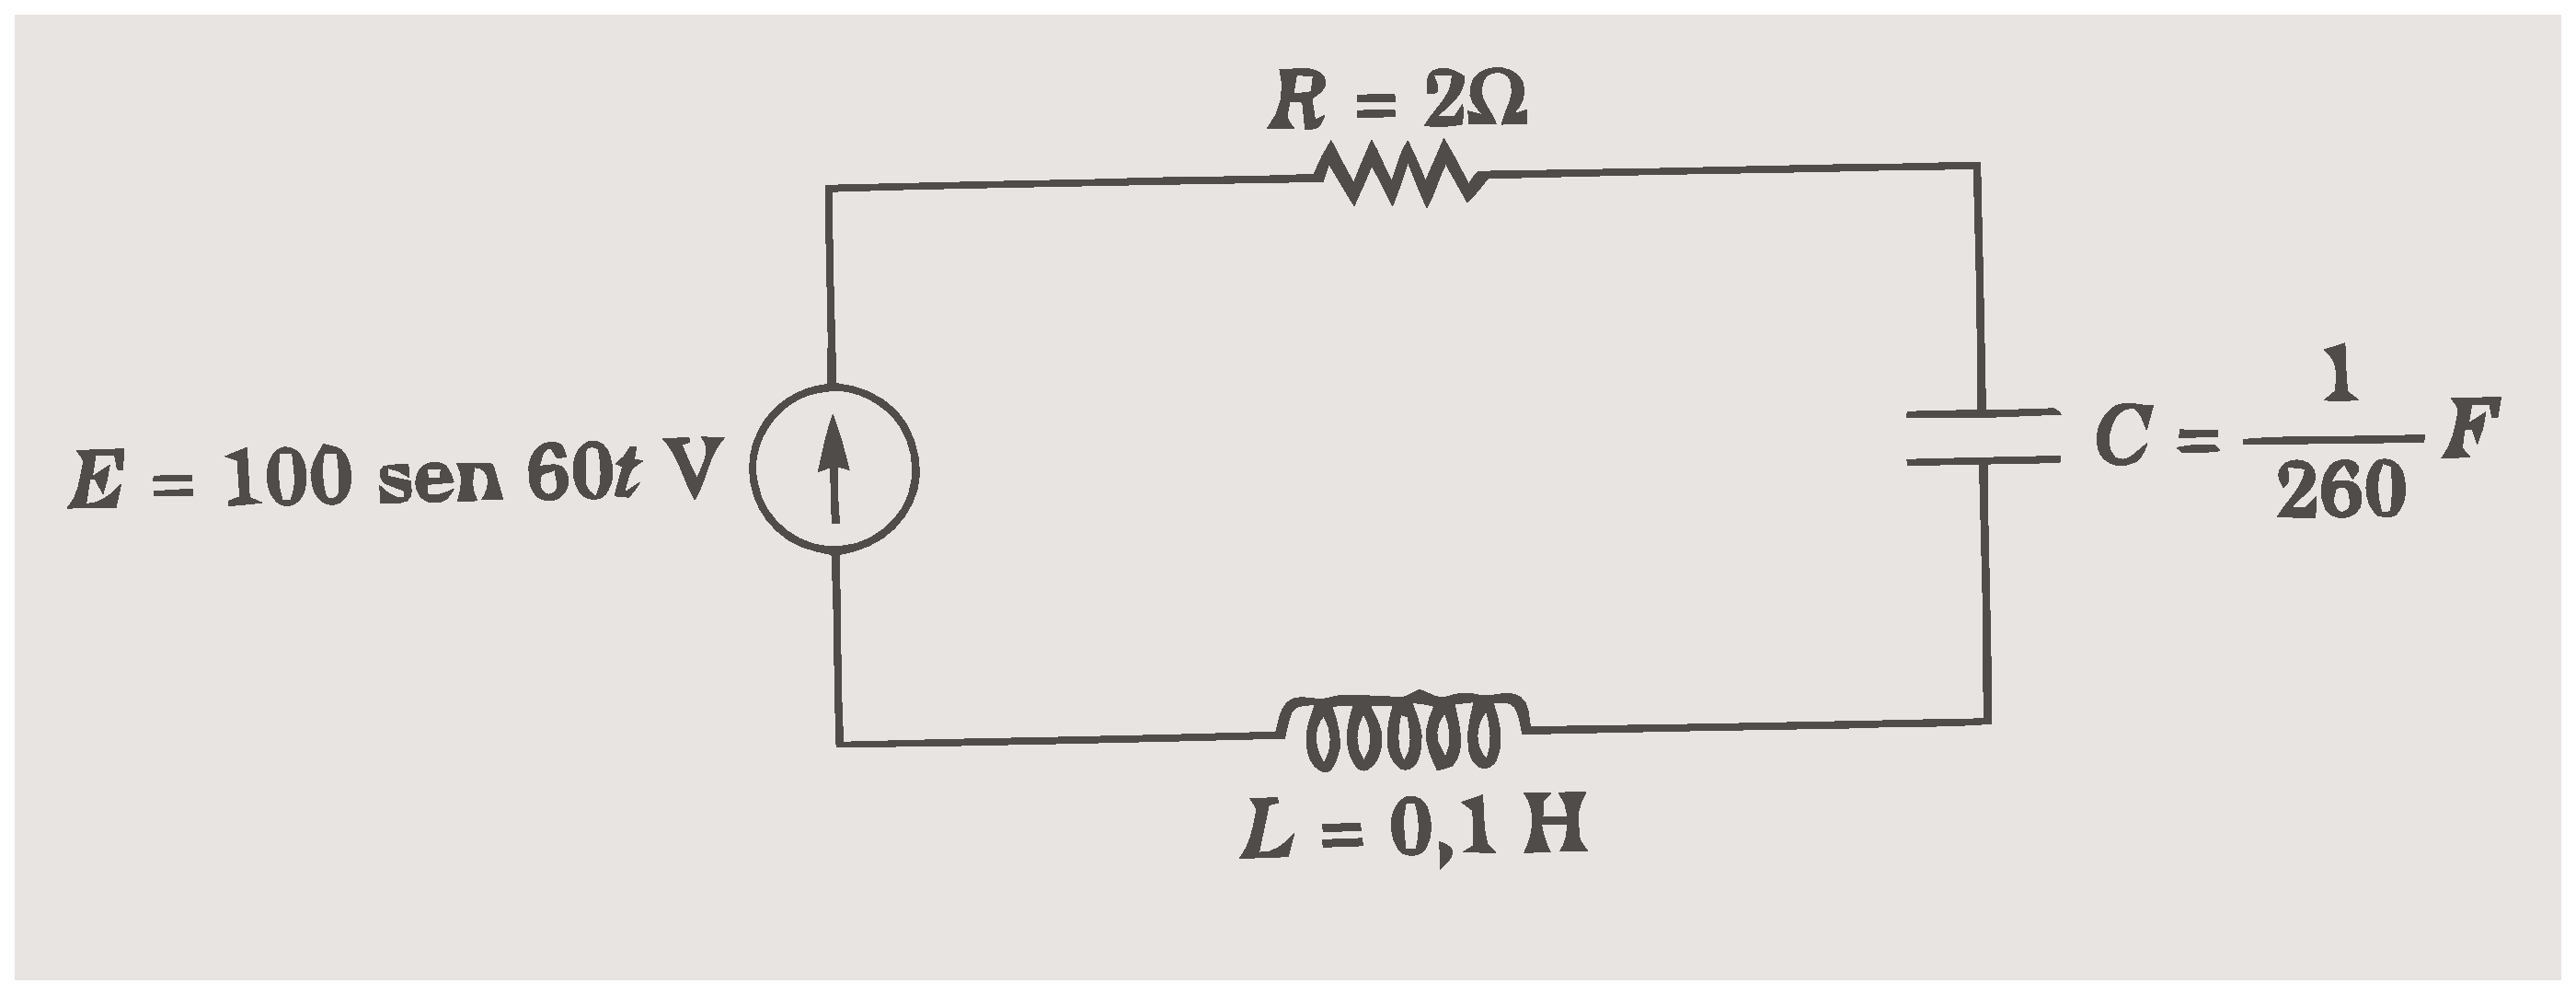
\includegraphics[width=0.5\textwidth]{ejerlc.eps}
\end{center}
y la soluci\'on de este P.V.I. se calcula siguiendo las instrucciones del siguiente rutero de \octave 
\begin{lstlisting}
c=1/260;
r=2;
l=0.1;
f=@(t,q) [q(2);(100*sin(60*t)-q(1)/c-r*q(2))/l];
[t,q]=ode45(f,[0,20],[0,0]);
plot(t,q(:,1),'-k');
xlabel('tiempo');
ylabel('carga');
title('Circuito RLC');
\end{lstlisting}
con lo cual se deermina la soluci\'on num\'erica
\begin{center}
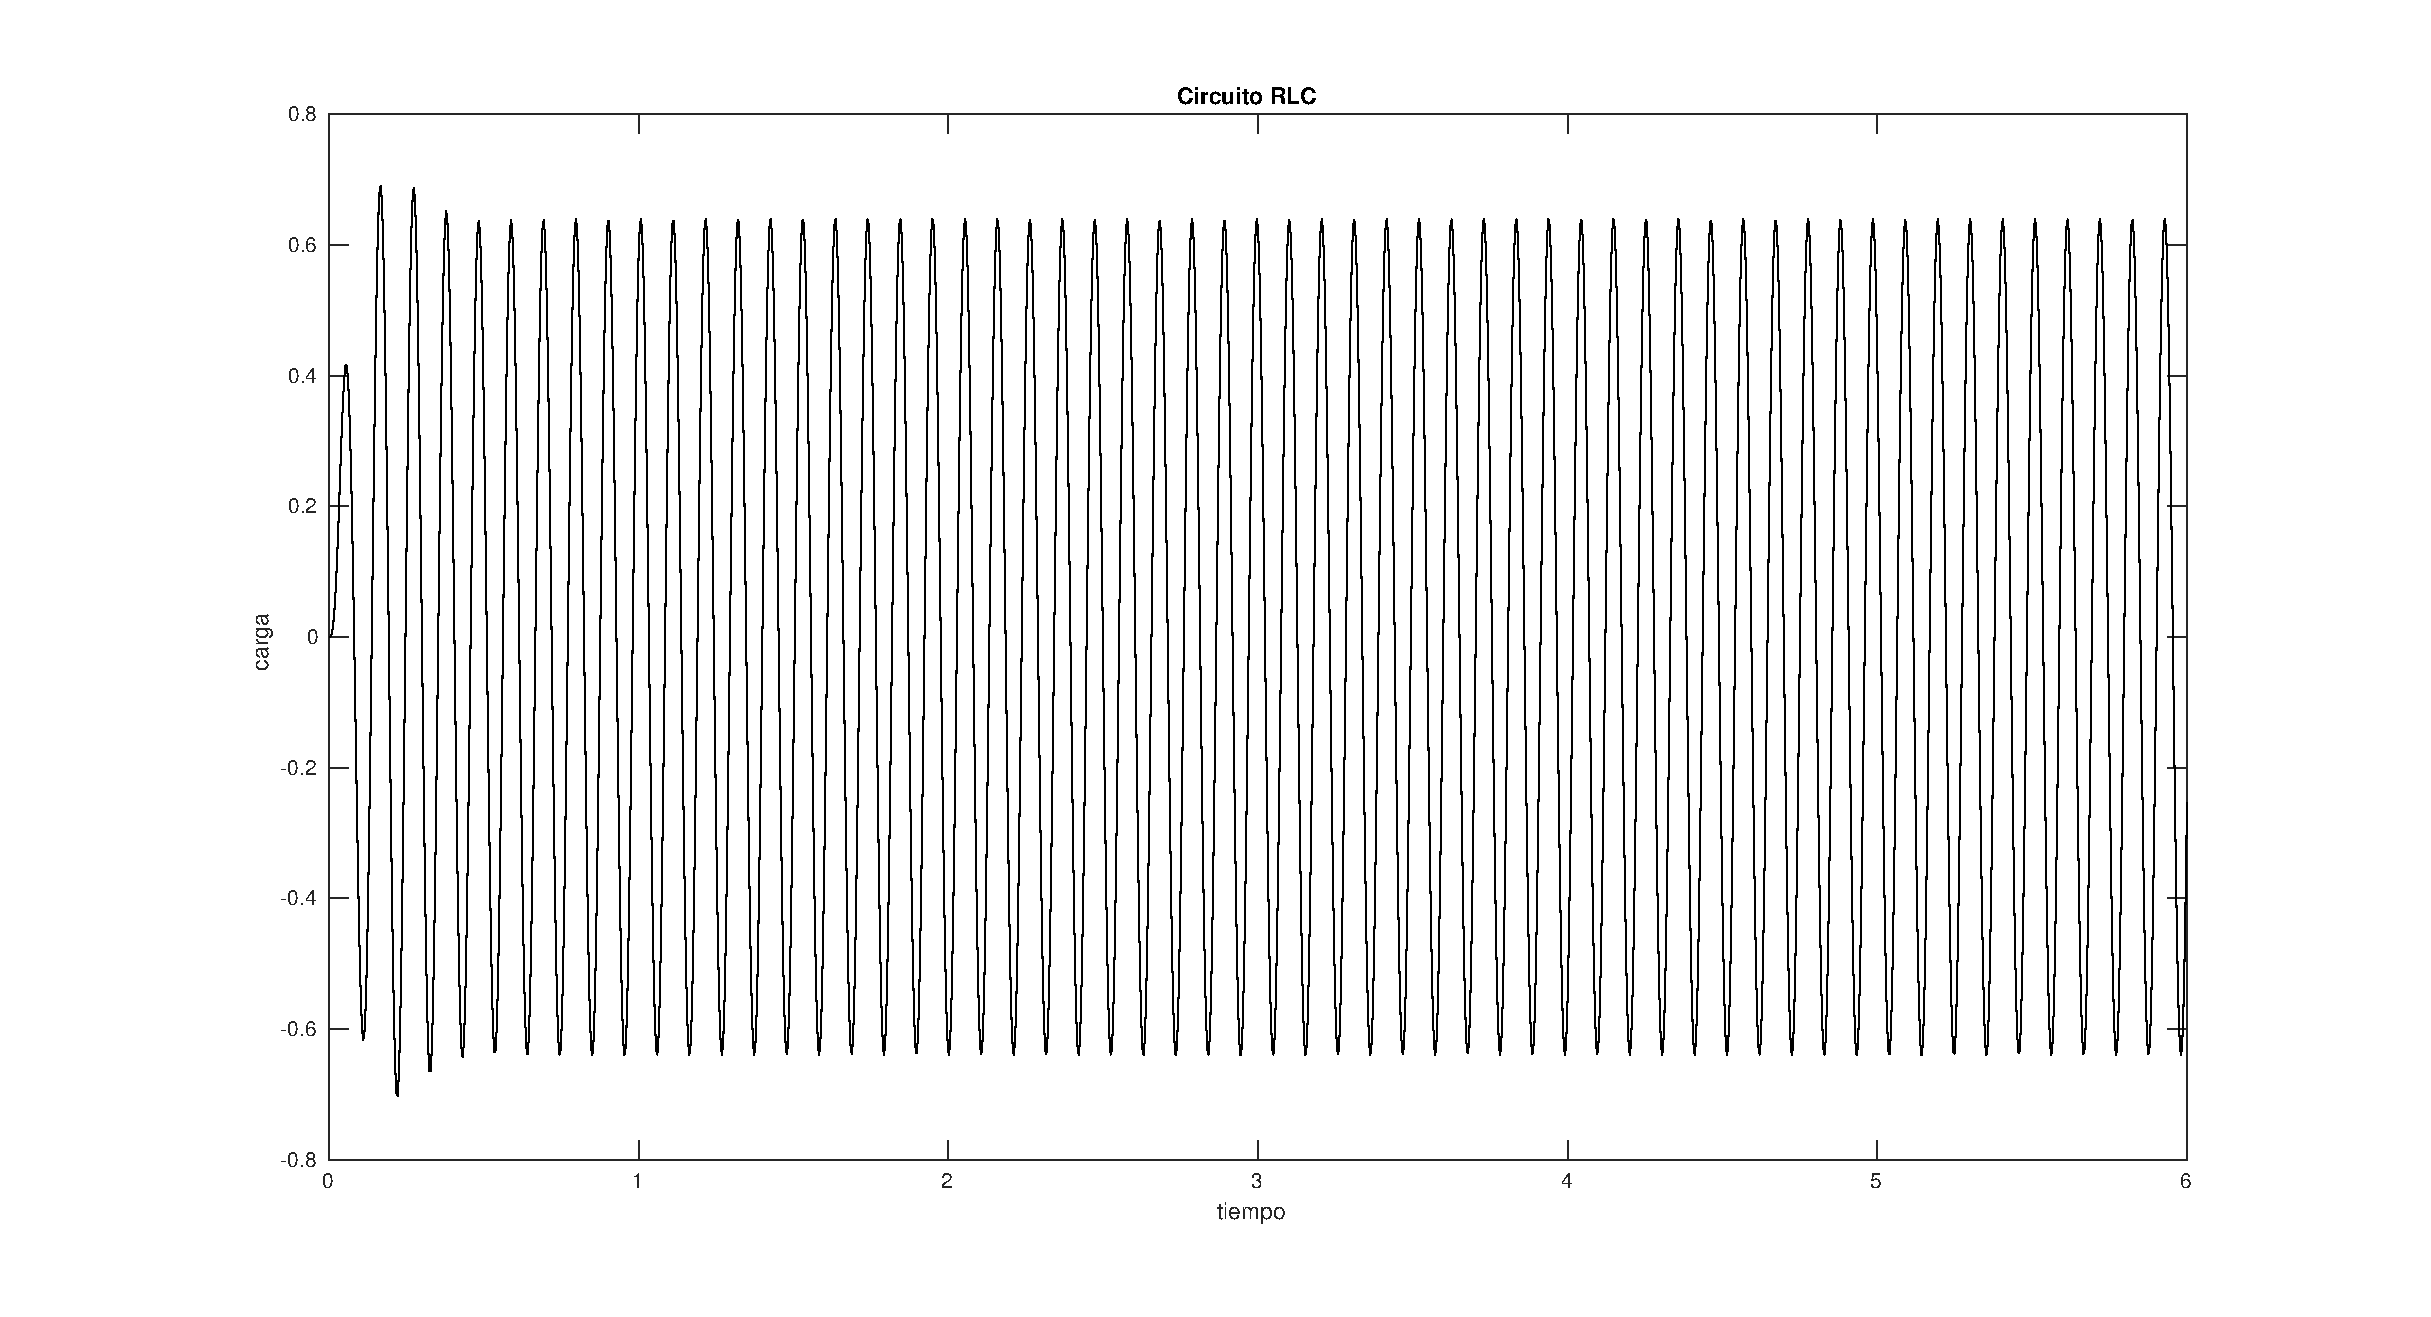
\includegraphics[width=0.85\textwidth]{eje6.eps}
\end{center}

%\subsubsection{Acoplamiento de sistemas masa-resorte-amortiguador}

\section{Ejercicios}
\begin{enumerate}
\item Programe el m\'etodo de Euler expl\'icito e impl\'icito para resolver los problemas
\begin{multicols}{2}
\begin{enumerate}
\item
$\begin{array}{rl|}
y'	&=\sen(2x)+y\\
y(0) &=0\\ \hline
\end{array}$
\item
$\begin{array}{rl|}
y'	&=\cos(3x)\\
y(0)&=0\\ \hline
\end{array}$
\item
$\begin{array}{rl|}
y''-y'-2y	&=\sen(2x)+y'\\
y(0)&=0\\
y'(0)&=0\\ \hline
\end{array}$
\end{enumerate}
\end{multicols}

\item La EDO
$$
y'=y^2-y^3
$$
modela el radio de una bola de fuego $y(t)$ en funci\'on del tiempo de combusti\'on. La idea es que este radio es proporcional a la superficie de la bola de fuego e inversamente proporcional a su volumen. Las llamas crecen r\'apidamente y, a medida que alcanzan su volumen final, dejan de crecer. 

Resuelva num\'ericamente el PVI
$$
\begin{array}{rl|}
y'  &=y^2-y^3 \\
y'(0) & = \delta \\ \hline
\end{array}
$$
considerando $\delta=0.1$, $\delta=0.05$, $\delta=0.001$ y $\delta=10 ^{-8}$.

\item Un circuito consta de una fuerza electromotriz alterna dada por
$$
E(t)=100\,sen(200t) \,[V]
$$
una resistencia de $40[\Omega]$, una bobina de $0.25[H]$ y un condensador de $4\times 10^{-4}[F]$ conectados en serie. Si la corriente inicial es cero y la carga inicial del capacitor es $0.01[C]$, hallar la expresi\'on de la corriente para $t>0$.

\item Un paracaidista de $80[kg]$ se suelta desde un avi\'on a una altura de $600[m]$. Despu\'es de $5[s]$ el paracaida se abre.

La altura del paracaidista, en funci\'on del tiempo, $y(t)[m]$ se modela por el PVI
$$
\begin{array}{rl|}
y'' 	& = -g+\frac{1}{m}\alpha(t),\\
y(0)	& = 600,\\
y'(0)	& 0,\\ \hline
\end{array}
$$
donde $g=9.81[m/s^2]$ es la aceleraci\'on de gravedad, $m=80[kg]$ es la masa del paracaidista y $\alpha(t)$ es la resistencia del aire, la cual es proporcional al cuadrado de la velocidad del paracaidista, pero esta cambia cuando el paraca\'idas se abre seg\'un
$$
\alpha(t)=
\begin{cases}
K_1\, y'(t)^2 , \quad \text{si} \quad t<5[s]\\
K_2\, y'(t)^2 , \quad \text{si} \quad t\geq 5[s]
\end{cases}.
$$
\begin{enumerate}
\item Calcule la soluci\'on anal\'itica en caida libre del paracaidista $(K_1=K_2=0)$. ?`Cu\'anto tiempo se demora el paracaidista en llegar a tierra? ?`Cu\'al es la velocidad del impacto?. Grafique la altura versus el tiempo.
\item Resuelva num\'ericamente considerando 
$$
K_1=1/15, \quad K_2=4/15.
$$
?`A qu\'e altura se abre el paraca\'idas? ?`Cuanto se demora en llegar al suelo? ?`Cu\'al es la velocidad del impacto? Grafique la altura versus el tiempo.
\end{enumerate}

%%%%%%%%%%
%%%%%%%%%%%%%%%%%%%%%


\item Consideremos un modelo, propuesto por Kermack y McKendrick en 1927 para describir la propagaci\'on de una epidemia en un grupo de $N$ personas en un per\'iodo de $T$ semanas.
Si $S(t)$ es el n\'umero de personas sanas al cabo de $t$ semanas, $E(t)$, el n\'umero de personas enfermas y $M(t)$, el de personas muertas, las ecuaciones que describen la evoluci\'on en el tiempo de $S(t)$, $E(t)$ y $M(t)$ son
\begin{align*}
S^{\prime} &= -c\,S\,E,\\
E^{\prime} &= c\,S\,E-m\,E,\\
M^{\prime} &= m\,E,
\end{align*}
donde $c$ y $m$ son las constantes que describen la rapidez con que la enfermedad se transmite
y la rapidez con que las personas enfermas mueren respectivamente.

Observe que
\[
\frac{\mbox{d}S}{\mbox{d}M} = \frac{\mbox{d}S}{\mbox{d}t}\frac{\mbox{d}t}{\mbox{d}M} =
-\frac c m S \Rightarrow S = S_0e^{-\frac c m M}
\]
si suponemos que el n\'umero inicial de personas muertas a causa de la enfermedad es cero
y $S_0$ denota el n\'umero inicial de personas sanas.

Adem\'as,
\[
S^{\prime} + E^{\prime} + M^{\prime} = 0 \Rightarrow S + E + M = \mbox{ constante },
\]
e igual al n\'umero de personas $N$ en el grupo considerado.

Con esto se tiene que
\[
E = N - S - M = N - S_0e^{-\frac c m M} - M
\]
y
\begin{equation}\label{pvi}\tag{PVI}
M^{\prime} = m\left(N - S_0e^{-\frac c m M} - M\right),\quad M(0) = 0,\quad t \in [0,\,10].
\end{equation}

\begin{enumerate}
\item Resuelva el problema de valores iniciales \eqref{pvi} con \texttt{ode45} suponiendo
$N = 3000$, $E(0) = 150$, $m = 1.8$ y $c = 0.001$.
Llame antes a \texttt{odeset} para hacer \texttt{AbsTol} igual a $10^{-8}$ y \texttt{RelTol} igual a $10^{-4}$.

\item Dibuje, en un mismo gr\'afico, el n\'umero de personas sanas, muertas
y enfermas en el per\'{\i}odo considerado (de 10 semanas).

\item ?`Al cabo de cu\'antas semanas aproximadamente se mantiene casi constante
el n\'umero de personas sanas, enfermas y muertas en el
grupo considerado?

\item ?`Cu\'al es el n\'umero de personas que ha muerto a causa de la enfermedad 8 semanas despu\'es
de comenzada la epidemia?
\end{enumerate}

\medskip

La resoluci\'on de PVI para sistemas de EDO se realiza mediante los mismos comandos. En tal caso, \verb+f(t,y)+ debe ser una funci\'on a valores vectoriales (es decir un \textbf{vector columna} de funciones) e \verb+y+ un \textbf{vector columna} de variables de la misma dimensi\'on. Adem\'as, la condici\'on inicial \verb+yo+ tambi\'en debe ser un \textbf{vector columna} de la misma dimensi\'on

\medskip


\item Considere un ecosistema simple consistente de conejos con una cantidad m\'as que suficiente de
alimento y zorros que depredan los conejos para su alimentaci\'on. Un modelo cl\'asico debido a
Volterra describe este ecosistema mediante el siguiente par de ecuaciones no lineales de primer
orden:

$$
\left\lbrace
\begin{array}{l}
\dfrac{dc}{dt}=2c-\alpha c z, \qquad c(0)=c_0,\\
\\
\dfrac{dz}{dt}=-z+\alpha c za, \qquad z(0)=z_0,\\
\end{array}\right.
$$

donde $t$ es el tiempo medido en a\~nos, $c=c(t)$ es el n\'umero de conejos y $z=z(t)$ el n\'umero de zorros, ambos en el instante $t$, y $\alpha$ es una constante positiva que mide la probabilidad de interacci\'on entre miembros de las dos especies.

\begin{enumerate}
\item Cuando $\alpha= 0$, conejos y zorros no interact\'uan. Resuelva la ecuaci\'on diferencial a lo largo de un a\~no en el caso en que inicialmente hay 100 animales de cada especie. Compruebe que en
tal caso los conejos hacen lo que mejor saben hacer, mientras los zorros se van muriendo de
hambre.

\item Calcule la evoluci\'on de ambas poblaciones a lo largo de 12 a\~nos en el caso en que
la constante de interacci\'on es $\alpha = 0{.}01$ y que la poblaci\'on inicial es de 300 conejos y 150 zorros. >Qu\'e conclusi\'on puede extraer en este caso?

\item Repita la simulaci\'on anterior pero con poblaciones iniciales de 15 conejos y 22 zorros. >Cu\'al es ahora la conclusi\'on?
\end{enumerate}



\item La litotricia extracorp\'orea por ondas de choque (LEC)
es un tratamiento no invasivo que utiliza un pulso ac\'ustico para romper los c\'alculos renales
(litiasis renal) y los c\'alculos biliares (piedras en la vejiga o en el h\'{\i}gado).

El LEC puede generar cierto da\~no colateral.
Las ondas de choque as\'{\i} como las burbujas (de aire) de cavitaci\'on formadas por la
agitaci\'on de la orina, pueden ocasionar da\~no a capilares,
he\-mo\-rra\-gia del parenquima renal o subcapsular.
Esto puede generar consecuencias a largo plazo tales como insuficiencia renal e hipertensi\'on.

El radio $R$ de las burbujas formadas despu\'es de $t$ microsegundos de comenzado el tratamiento es $R(t) = 3\times 10^{-6} r(t)$ metros,
donde $r$ es la soluci\'on
a la siguiente ecuaci\'on diferencial, propuesta en 1998 por Howle, Shearer y Zhong,
\begin{equation}\label{bubblepvi}\tag{LEC}
rr^{\prime\prime} + \frac 3 2 \left(r^{\prime}\right)^2 = r^{-3\gamma} - 1,
\quad r(0) = A,\;r^{\prime}(0) = 0
\end{equation}
en la que $\gamma = 1.4$ es el exponente adiab\'atico.

\begin{enumerate}
\item Convierta \eqref{bubblepvi} a un sistema de ecuaciones diferenciales de primer
orden.
\item Resuelva el problema de valores iniciales resultante con $t \in [0,\,20]$
y suponiendo $A = 2.5$.
\item Grafique la aproximaci\'on resultante y observe
que es una funci\'on peri\'odica, ?`cu\'al es el per\'{\i}odo aproximado de la misma?
?`Entre qu\'e valores oscila el radio $R$ de la burbuja?
\end{enumerate}



\item Considere el problema de valores iniciales
\begin{align*}
y^{\prime}(x) &= 100(1-y(x)),\; x \in [0,\,5],\\
y(0) &= 2.
\end{align*}
\begin{enumerate}
\item Resuelva este problema con \texttt{ode45} y \texttt{ode15s}
tomando \texttt{AbsTol} = 1e-6 y \texttt{RelTol} = 1e-4.
?`En cu\'antos subintervalos divide \texttt{ode45} el intervalo de integraci\'on $[0,\,5]$
para resolver este problema?
?`En cu\'antos lo divide \texttt{ode15s}?
Observe que \texttt{ode15s} necesita dividir $[0,\,5]$ en muchos menos subintervalos
que \texttt{ode45}, a pesar de que las tolerancias con que ambos m\'etodos calculan son las mismas.
Este comportamiento es t\'{\i}pico de problemas \emph{stiff}.

\item Grafique los tama\~nos de paso generados por ambos m\'etodos y la soluci\'on
exacta a este problema $y(t) = e^{-100\,t} + 1$.

\noindent Observe que la soluci\'on exacta de este problema var\'{\i}a rapidamente desde el valor inicial
hasta un valor cercano a 1, pero para $t \ge 0.1$ se mantiene casi constante.
Es de esperarse que a partir de $0.1$ un m\'etodo num\'erico para resolver este problema tome
en $[0,\,0.1]$ tama\~nos de paso peque\~nos, para poder reproducir la variaci\'on de la soluci\'on exacta, pero
a partir de $0.1$ use tama\~nos de paso mucho mayores.

\noindent Sin embargo, en los gr\'aficos de los tama\~nos de paso usados por \texttt{ode45} y \texttt{ode15s},
s\'olo \texttt{ode15s} exhibe el comportamiento esperado. El comportamiento de \texttt{ode45} es el t\'{\i}pico
de m\'etodos no adecuados para resolver problemas \emph{stiff} al usarse para resolver problemas \emph{stiff}.
\end{enumerate}

\item Consideremos el Problema de Valores Iniciales
\begin{equation*}
x^{\prime} = -3t\,x^2 + \frac{1}{1+t^3},\quad x(0) = 0,\quad t \in [0,\,5]
\end{equation*}
cuya soluci\'on exacta es
\[
x(t) = \frac{t}{1+t^3}.
\]
\begin{enumerate}
\item Resuelva el problema con \texttt{ode45} y los pares de valores de
\texttt{AbsTol} y \texttt{RelTol} en la tabla \ref{tab:ej2} y compl\'etela.

\begin{table}[h]
\begin{center}
\begin{tabular}{|c|c|c|}\hline
\texttt{RelTol} & \texttt{AbsTol} & $\max_{i} |x_i - x(t_i)|$\\\hline
\texttt{1e-2} & \texttt{1e-4} & \\\hline
\texttt{1e-3} & \texttt{1e-5} & \\\hline
\texttt{1e-4} & \texttt{1e-6} & \\\hline
\texttt{1e-5} & \texttt{1e-7} & \\\hline
\end{tabular}
\end{center}
\caption{Comportamiento de ode45}\label{tab:ej2}
\end{table}

\noindent Observe que no siempre se cumple que $\max_i |x_i - x(t_i)| \le $ \texttt{AbsTol}, sin embargo, dis\-mi\-nu\-yen\-do los valores de \texttt{AbsTol} y \texttt{RelTol} la soluci\'on calculada
por \texttt{ode45} se acerca a la soluci\'on exacta del problema.

\item Con los valores devueltos en \'ultimo llamado a \texttt{ode45}
grafique la soluci\'on exacta y los tama\~nos de paso con los que ha calculado
\texttt{ode45}, es decir, si usted llam\'o a \texttt{ode45} de este modo

\medskip
\begin{lstlisting}
[t,x] = ode45(...)
\end{lstlisting}
\medskip

\noindent escriba

\medskip
\begin{lstlisting}
figure(1)
plot(t,t./(1+t.^3))
figure(2)
plot(t(1:end-1),t(2:end)-t(1:end-1))
\end{lstlisting}
\medskip

\noindent Observe que en el tramo en el que la soluci\'on exacta del problema var\'{\i}a m\'as r\'apidamente los tama\~nos de paso con los que calcula \texttt{ode45} son m\'as peque\~nos.
\end{enumerate}


\item Considere el siguiente Problema de Valores Iniciales:

$$
\left\{ \begin{array}{l}
 x'=3 \sen(t)x+2ty+1 \qquad t\in[0, 1{.}5]\\
y''=2x+t^2y'-5y+e^t\qquad t\in[0, 1{.}5]\\
x(0)=0,\quad y(0)=2,\quad y'(0)=0\\
\end{array}\right.
$$

\noindent donde $x=x(t)$ e $y=y(t)$. Para resolver este problema, utilizaremos el M\'etodo de Euler impl\'icito, en cual considera una partici\'on del intervalo $[0, 1{.}5]$ en $N$ subintervalos de tama\~no $h$, donde:
$$t_i=(i-1)h,\,\,\,i=1,\ldots,N+1\qquad \textrm{con} \qquad h=\dfrac{1{.}5}{N}. $$
El algoritmo del m\'etodo de Euler impl\'icito queda:

\begin{center}
\begin{tabular}{|l|}
\hline
Dado $\boldsymbol{y}_1$\\
Para $i=1,\ldots,N$\\
\quad\begin{tabular}{|l}
  $\boldsymbol{y}_{i+1}=\boldsymbol{y}_i+h\boldsymbol{F}(t_{i+1},\boldsymbol{y}_{i+1})$ \\
\end{tabular}\\[4pt]
\hline
\end{tabular}
\end{center}

\begin{enumerate}

\item Utilizando un cambio de variables apropiado, escriba el PVI asociado como un sistema de EDO de primer orden, con sus respectivas condiciones iniciales.

\item Escriba el sistema de ecuaciones lineales que define el esquema de Euler impl\'icito para las EDO del item anterior:

\item Escriba un programa tipo rutero en ambiente \octave que realice las siguientes tareas:

\begin{enumerate}
\item Resuelva el problema utilizando el esquema de Euler impl\'icito, considerando $N=100$.

\item Resuelva el problema utilizando el comando \texttt{ode45}, utilizando la misma partici\'on definida en el item anterior.

\item En una misma figura grafique $x(t)$ obtenidos por el m\'etodo de Euler impl\'icito y el comando \texttt{ode45}.
\item En otra figura grafique $y(t)$ obtenidos por el m\'etodo de Euler impl\'icito y el comando \texttt{ode45}.
\end{enumerate}

\item Un proyectil de masa $m$ se arroja desde un punto del plano $(x0, y0)$, con una velocidad inicial dada por el vector $(v_0^x,v_0^y)$.  La trayectoria del proyectil se
rige por las ecuaciones dadas por la segunda ley de Newton:
$$
\begin{array}{cc}
mx'' &= −\gamma v^x\\
my'' &= −mg − \gamma v^y
\end{array}
$$
donde $g$ es la aceleraci\'on de gravedad $g = 9.81 [m/s^2]$, y $\gamma$ es una constante de roce con el
medio en que se realiza el lanzamiento. Formule este problema en forma de un sistema de orden
uno.

Considerando $ m = 10[Kg]$ y $\gamma = 0.2[Kg/s]$ y suponiendo que el proyectil se lanza desde $30[m]$
de altura con una velocidad inicial horizontal de $40 [m/s]$, \textquestiondown Qu\'e distancia recorre antes de tocar el piso?

Haga un programa que permita responder esta pregunta, utilizando el m´etodo de Euler impl\'icito para resolver el sistema.

\end{enumerate}


%\medskip
%\centerline{\textsc{Problemas de Valores de Contorno}}
%\medskip
%
%\begin{description}
%\item[\textbf{Ejercicio 7.}] Considere el siguiente Problema de Valores de Contorno:
%
%$$
%\textrm{PVC}\,
%\left\{ \begin{array}{l}
% u'' + 2(1-x^2)u'+u^2=1 \qquad x \in [-1,1]\\
%u(-1)=0,\quad u(1)=-0{.}1\\
%\end{array}\right.
%$$
%
%Para resolver este problema, utilizaremos el M\'etodo de \emph{Shooting} (visto en clases),
%el cual considera el siguiente Problema de Valores Iniciales asociado:
%
%$$
%\textrm{PVI}\,
%\left\{ \begin{array}{l}
% u'' + 2(1-x^2)u'+u^2=1 \qquad x \in [-1,1]\\
%u(-1)=0,\quad u'(-1)=z\\
%\end{array}\right.
%$$
%
%\noindent donde $z \in \mathbb{R}$. La idea es encontrar un valor $\bar{z}$ de modo que la soluci\'on del PVI asociado, $u_z$, coincida con la condici\'on de contorno en el extremo derecho del PVC, esto es:
%
%$$u_z(1)=-0{.}1$$
%
%\noindent lo que equivale a encontrar la soluci\'on a la ecuaci\'on no lineal $E(z)=0$, donde
%
%$$E(z)=u_z(1)+0{.}1$$
%
%%Condsideraremos $\varepsilon=1$, $\alpha=0$ y $\beta=-0.1$
%
%\begin{enumerate}
%
%\item[7.1] Utilizando un cambio de variables apropiado, escriba el PVI asociado como un sistema de EDO de primer orden, con sus respectivas condiciones iniciales.
%
%\item[7.2] Escriba un programa tipo \verb"function"  en ambiente \textsc{Matlab} que tenga como entrada el un valor $z$ y como salida el valor de la funci\'on $E$ evaluada en este valor $z$. Para ello, tenga en cuenta que su funci\'on debe resolver num\'ericamente el PVI asociado (utilizando \verb"ode45") con este valor de $z$.
%
%\item[7.3] Escriba un programa tipo rutero en ambiente \textsc{Matlab} que realice las siguientes tareas:
%
%\begin{enumerate}
%\item Resuelva la ecuaci\'on no lineal $E(z)=0$, con $E(z)$ definido en el item anterior. Utilice el comando \verb"fzero", con $z_0=1$ como una aproximaci\'on inicial. Su programa debe mostrar el valor de la soluci\'on $\bar{z}$:
%
%    \begin{center}
%\begin{tabular}{|l|c|}
%\hline $\bar{z}$ & \ \hskip3.cm\ \\
%\hline
%\end{tabular}
%
%\smallskip
%(Complete la tabla anterior)
%\end{center}
%
%\item Con el valor de $\bar{z}$ encontrado en el item anterior, grafique en un mismo gr\'afico $u$ y $u'$, las soluciones del Problema de Valores de Contorno.
%
%\end{enumerate}



%%%%%%%%%%%%%%%%%%%%%



%%%%%%%%%%%%%

\end{enumerate}

% \newpage
% \section{Deflexiones de una viga}

% Muchas estructuras se construyen mediante vigas o travesa\~{n}os y éstas se distorsionan bajo su propio peso o por influencia de algunas fuerzas externas.
%      \begin{figure}[htp]
%       \begin{center}
% 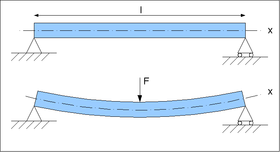
\includegraphics[width=0.5\textwidth]{./viga.png}
%       \caption{\sl Deflexi\'on en una viga.}
%       \end{center}
%       \end{figure}
      
% Supongamos que una viga de longitud $L$ es homog\'enea en su composici\'on y que tiene cortes transversales uniformes a su largo. En ausencia de cualquier carga en la viga, incluyendo su propio peso, la viga describir\'a una recta llamada eje de simetr\'ia. Si una carga se aplica a la viga, en forma perpendicular al eje de simetr\'ia, esta experimenta una deformaci\'on. La curva que describe la deformaci\'on de cada punto respecto al eje de simetr\'ia es llamada \textbf{curva de deflexiones} o \textbf{curva el\'astica}. En cierto sentido, la curva de deflexiones aproxima la forma de la viga.
%      \begin{figure}[htp]
%       \begin{center}
% 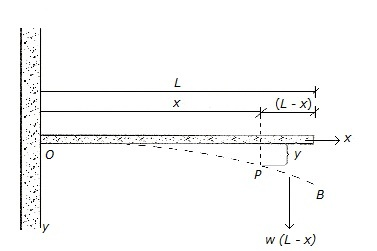
\includegraphics[width=0.5\textwidth]{./viga1.jpg}
%       \caption{\sl Sistema coordenado en una viga y curva de deflexi\'on.}
%       \end{center}
%       \end{figure}

% Suponga que el eje $x$ coincide con el eje de simetr\'ia de una viga y que la deflexi\'on es medida como funci\'on de la posici\'on del eje $x$, digamos $y(x)$. En la teor\'ia de elasticidad se tiene que
% $$
% EI y^{(iv)}(x)=w(x),
% $$
% donde $E$ es el m\'odulo de Young, $I$ es el momento de inercia de un corte transversal de la viga, ambas constantes que dependen de la geometr\'ia y material de la viga, mientras que $w(x)$ es la carga que hay en el punto $x$ de la viga.

% La condiciones de contorno para la curvatura el\'astica cumplen un rol importante, y podemos clasificarlas en tres tipos de vigas

% \begin{center}
% \begin{tabular}{||c|c||}
% \textbf{Extremos en la viga} & \textbf{Condiciones de frontera}  \\
% \hline
% Empotrados 	& $y=0$, $y'=0$ 	\\                                    
% Libres		& $y''=0$, $y'''=0$	\\
% Apoyados	& $y=0$, $y''=0$	 
% \end{tabular}
% \end{center}

% \begin{enumerate}
% \item
% Encuentre la soluci\'on num\'erica que describa la deflexi\'on de una viga de largo $L$ empotrada en ambos extremos sujeta a una carga constante $w_0$.

% Grafique la deflexi\'on de vigas de largo $1$ , $10$ y $100$ cuando $w_0=24\times 10^{-4}$.

% \item 
% Encuentre la soluci\'on num\'erica que describa la deflexi\'on de una viga de largo $L$ empotrada en un extremo y libre en el otro, sujeta a una carga constante $w_0$.

% Grafique la deflexi\'on de vigas de largo $1$ , $10$ y $100$ cuando $w_0=24\times 10^{-5}$.

% \item 
% Encuentre la soluci\'on num\'erica que describa la deflexi\'on de una viga de largo $L$ empotrada en ambos extremos, sujeta a una carga $w(x)=w_0 x$.

% Grafique la deflexi\'on de vigas de largo $1$ , $10$ y $100$ cuando $w_0=24\times 10^{-1}$.
% \end{enumerate}

\vfill
\hfill Revisado a Semestre 2018--1
\end{document}
